\chapter{Componentes triconexas}

Para esta parte se utilizan los conceptos generados por \citep{hopcroft1973} y mejorados por \citep{Gutwenger2000ALT}.

\section{Dividir una gráfica en componentes triconexas}

\subsection{Introducción}

\paragraph{}
Las propiedades de conectividad de las gráficas forman una parte importante de la teoría de gráficas. En \citep{hopcroft1973} se considera el problema de separar una gráfica en sus componentes triconexas. Un algoritmo para esto es de utilidad para analizar circuitos eléctricos \citep{1083313} , para determinar si una gráfica es plana \citep{10893101} y para determinar cuando dos gráficas planas son isomorfas \citep{Hopcroft1972}. Un algoritmo para planaridad puede ser usado en el diseño de tablas de circuitos; un algoritmo para isomorfismo de gráficas planas puede ser usado para probar el isomorfismo estructural de compuestos químicos \citep{Lederberg1964DENDRAL64AS} y en nuestro caso para ayudar a clasificar gráficas de Dynkin de tipo $\DynD_{n}$.\\

Una técnica que se ha utilizado para resolver problemas de conectividad es el recorrido primero en profundidad. En \citep{4569669} y \citep{efalgm}, se aplica la búsqueda primero en profundidad para obtener algoritmos eficientes para determinar las componentes biconexas de una gráfica no dirigida y para determinar las componentes fuertemente conexas de una gráfica dirigido. El método también se ha utilizado en un algoritmo eficiente para pruebas de planaridad (\citep{tarjan1971efficient}, \citep{ept}) y en un algoritmo para encontrar dominadores en un grafo de flujo \citep{Tarjan1974FindingDI}. Aquí se aplica la búsqueda primero en profundidad al problema de encontrar las componentes triconexas de una gráfica. Los métodos antiguos para determinar estos componentes requieren $\Theta\left(V^{3}\right)$ pasos o más, si el la gráfica tiene $V$ vértices(\citep{1083313}, \cite{1082941}). El algoritmo descrito aquí requiere sustancialmente utilizamos la combinación de los artículos \citep{hopcroft1973} y mejorados por \citep{Gutwenger2000ALT}.\\

Se usa la siguiente notación para especificar límites: si $f$ y $g$ son funciones de $x$, digamos que $f\left(x\right)$ es $\Theta\left(g\left(x\right)\right)$ si, para algunas constantes $k_{1}$ y $k_{2}$, $\left|f\left(x\right)\right| \leq k_{1}\left|g\left(x\right)\right| + k_{2}$ para todo $x$\\

\subsection{Gráficas, conectividad y busqueda en profundidad}

Las definiciones utilizadas aquí se ven \citep{busacker1965finite} y \citep{harary1971graph}. Las componentes triconexas pueden definirse de varias maneras, todas más o menos equivalentes. Los resultados a continuación, se dan sin prueba, siguen de Saunders Maclaine \citep{mac-lane-1937}; estas definiciones se modifican un poco para hacerlos más adecuadas para aplicaciones computacionales.\\

\paragraph{}
Una gráfica $G = \left(\mathscr{V},\mathscr{E}\right)$ consiste de un conjunto $\mathscr{V}$ que contiene $\mathrm{V}$ vértices y un conjunto $\mathscr{E}$ que contiene $\mathrm{E}$ aristas. Si $\mathscr{E}^{`}$ es un conjunto de aristas en $G$, $\mathscr{V}\left(\mathscr{E}^{`}\right)$ es el conjunto de vértices que inciden a uno o más aristas en $\mathscr{E}^{`}$. Si $S$ es un conjunto de vértices en $G$, $\mathscr{E}\left(\mathscr{S}\right)$  es el conjunto de aristas incidentes a al menos un vértice en $S$.

\paragraph{}
Un \textbf{camino} $p:v \overset{\ast}{\Rightarrow} w$ en $G$ es una secuencia de vértices y aristas que van de $v$ a $w$. Un camino es simple si todos sus vértices son distintos. Un camino $p:v \overset{\ast}{\Rightarrow} v$ es un \textbf{ciclo} si todas las aristas son distintas y el único vértice que se repite en $p$ es $v$ y este está al principio y al final de la secuencia de vértices. Un gráfica no dirigida(sin dirección) es conexa(esta conectada) si para cada par de vértices $(v, w)$ existe un camino entre $(v,w)$. Sea $G= \left(\mathscr{V},\mathscr{E}\right)$ y sea $G' =  \left(\mathscr{V}^{`},\mathscr{E}^{`}\right)$ dos gráficas tales que $\mathscr{V}^{`}\subseteq\mathscr{V}$ y $\mathscr{E}^{`}\subseteq \mathscr{E}$ entonces $G^{`}$ es una subgráfica de $G$. Una gráfica con exactamente dos vértices $v,w$ y uno o más aristas $\left(v,w\right)$ se le dice \textbf{enlace}.

\paragraph{}
Un árbol $T$ (dirigido, enraizado) es una gráfica dirigida cuya versión no dirigida es conexa, que tienen un vértice (llamado raíz) y en el que cualquier par de vértices están conectados por exactamente un camino. La relación ``$(v, w)$ es una arista de $T$'' se denota por $v \rightarrow w$. La relación ``hay un camino de $v$ a $w$ en $T$'' se denota por $v \overset{\ast}{\rightarrow}  w$. Si $v \rightarrow w$, donde $v$ es el padre de $w$, y $w$ es un hijo de $v$.Si $v \overset{\ast}{\rightarrow} w$, entonces v en un ancestro de w y w es un descendiente de v. El conjunto de descendientes de un vértice $v$ se denota por $D\left(v\right)$. Todo vértice es ancestro y descendiente de sí mismo. Si $G$ es una gráfica no dirigida, un árbol $T$ es un \textbf{árbol generador} de $G$ si $T$ es un subgráfica de $G$ y $T$ contiene todos los vértices de $G$.

\paragraph{}
Sea $P$ una gráfica no dirigida que consta de dos conjuntos disjuntos de aristas, denotados por $v \rightarrow w$ y $v \rule[1mm]{.1cm}{0.4pt} \rightarrow w$. Supongamos que $P$ satisface las siguientes propiedades:
\begin{enumerate}
\item La subgráfica $T$ que contiene las aristas $v \rightarrow w$ es un árbol generado de $P$.
\item Si $v~ \rule[1mm]{.2cm}{0.4pt} \rightarrow w$, entonces $w \overset{\ast}{\rightarrow}  v$. Es decir, cada arista que no está en el árbol generador $T$ de $P$ conecta el vértice $w$ con uno de sus ancestros $v$ en $T$.
\end{enumerate}
Entonces a $P$ llamaremos árbol de recorrido. Las aristas $v~ \rule[1mm]{.2cm}{0.4pt} \rightarrow w$ las llamaremos aristas de retroceso de $P$.

\paragraph{}
Un gráfica conexa $G$ es \textbf{biconexa} si por cada tripleta de vértices distintos $v$, $w$ y $a$ en $V$, hay un camino $p: v \overset{\ast}{\rightarrow} w$ tal que $a$ no está en el camino $p$. Si hay una tripleta distinta $v$, $w$, $a$ tal que $a$ está en cada camino de  $p :v  \overset{\ast}{\rightarrow} w$, entonces se dice que  $a$ es un \textbf{punto de separación} (o  \textbf{punto de articulación}) de $G$. Podemos particionar las aristas de $G$ de manera que dos aristas están en el mismo bloque de la partición si y sólo si pertenecen a un \textbf{ciclo}. Sea $G_{i} =  \left(V_{i}, E_{i}\right)$ donde $E_{i}$ es el conjunto de aristas en el $i$-ésimo bloque de la partición, y $V_{i} = V\left(E_{i}\right)$. Entonces lo siguiente se cumple:
\begin{enumerate}
\item Cada $G_{i}$ es biconexa.
\item Ningún $G_{i}$ es una subgráfica propia de una subgráfica biconexa de $G$.
\item Cada vértice de $G$ que no sea un punto de articulación de $G$ está exactamente una vez entre los $V_{i}$ y cada punto de articulación está al menos dos veces.
\item Para cada $i, j, i \neq j, V_{i} \cap V_{j}$ contiene como máximo un vértice; además, este el vértice (si existe) es un punto de articulación.
\end{enumerate}
Los subgráficas $G_{i}$ de $G$ se denominan \textbf{componentes biconexas} de $G$. Las componentes biconexas de $G$ son únicas.

\begin{definition}
Sea $G = (V, E)$ una gráfica y sea $H = (W, F)$ una subgráfica de $G$, definimos una relación de equivalencia sobre $E − F$ como sigue:
 \begin{enumerate}
  \item $\forall e \in E - F$, $e \tilde{=} e$
  \item $\forall e, f \in E - F$ con $e: a_{1} \rule[1mm]{.1cm}{0.4pt} b_{1}$ y $f: a_{2} \rule[1mm]{.1cm}{0.4pt} b_{2}$, entonces $e \tilde{=} f$ si y solo si existe un camino de los siguientes tipos:
  \begin{itemize}
   \item $a_{1} \tikz[baseline=-0.1ex]\draw (0,0.05) -- (0.3,0.05); b_{1} \tikz[baseline=-0.1ex]\draw (0,0.05) -- (0.3,0.05); v_{1} \tikz[baseline=-0.1ex]\draw (0,0.05) -- (0.3,0.05); v2 \tikz[baseline=-0.1ex]\draw (0,0.05) -- (0.3,0.05); \cdots \tikz[baseline=-0.1ex]\draw (0,0.05) -- (0.3,0.05); v_{k} \tikz[baseline=-0.1ex]\draw (0,0.05) -- (0.3,0.05); a_{2} \tikz[baseline=-0.1ex]\draw (0,0.05) -- (0.3,0.05); b_{2}$ tal que $b_{1}, v_{1}, \ldots, v_{k}, a_{2} \notin W$
   \item $a_{1} \tikz[baseline=-0.1ex]\draw (0,0.05) -- (0.3,0.05); b_{1} \tikz[baseline=-0.1ex]\draw (0,0.05) -- (0.3,0.05); v_{1} \tikz[baseline=-0.1ex]\draw (0,0.05) -- (0.3,0.05); v2 \tikz[baseline=-0.1ex]\draw (0,0.05) -- (0.3,0.05); \cdots \tikz[baseline=-0.1ex]\draw (0,0.05) -- (0.3,0.05); v_{k} \tikz[baseline=-0.1ex]\draw (0,0.05) -- (0.3,0.05); b_{2} \tikz[baseline=-0.1ex]\draw (0,0.05) -- (0.3,0.05); a_{2}$ tal que $b_{1}, v_{1}, \ldots, v_{k}, b_{2} \notin W$
   \item $b_{1} \tikz[baseline=-0.1ex]\draw (0,0.05) -- (0.3,0.05); a_{1} \tikz[baseline=-0.1ex]\draw (0,0.05) -- (0.3,0.05); v_{1} \tikz[baseline=-0.1ex]\draw (0,0.05) -- (0.3,0.05); v2 \tikz[baseline=-0.1ex]\draw (0,0.05) -- (0.3,0.05); \cdots \tikz[baseline=-0.1ex]\draw (0,0.05) -- (0.3,0.05); v_{k} \tikz[baseline=-0.1ex]\draw (0,0.05) -- (0.3,0.05); a_{2} \tikz[baseline=-0.1ex]\draw (0,0.05) -- (0.3,0.05); b_{2}$ tal que $a_{1}, v_{1}, \ldots, v_{k}, a_{2} \notin W$
   \item $b_{1} \tikz[baseline=-0.1ex]\draw (0,0.05) -- (0.3,0.05); a_{1} \tikz[baseline=-0.1ex]\draw (0,0.05) -- (0.3,0.05); v_{1} \tikz[baseline=-0.1ex]\draw (0,0.05) -- (0.3,0.05); v2 \tikz[baseline=-0.1ex]\draw (0,0.05) -- (0.3,0.05); \cdots \tikz[baseline=-0.1ex]\draw (0,0.05) -- (0.3,0.05); v_{k} \tikz[baseline=-0.1ex]\draw (0,0.05) -- (0.3,0.05); b_{2} \tikz[baseline=-0.1ex]\draw (0,0.05) -- (0.3,0.05); a_{2}$ tal que $a_{1}, v_{1}, \ldots, v_{k}, b_{2} \notin W$
  \end{itemize}
 \end{enumerate}
\end{definition}

\paragraph{}
Si $H = \{\{a, b\}, \emptyset \}$, las clases de equivalencia son llamadas clases de separación relativas al par $\{a, b\}$.
\begin{definition}
Sean $S_{1}, S_{2}, \ldots, S_{k}$, las clases de separación relativas al par $\left(a, b\right)$. Si existe una partición $\left(A, b\right)$ de $\{1, 2, \ldots, k\}$ tal que $\left| E_{1} = \bigcup_{i \in A} S_{i}\right| \geq 2$ y $\left|E_{2} = \bigcup_{j \in B} S_{j}\right| \geq 2$ decimos que $\{a, b\}$ es un par de separación. Veamos esto en el siguiente ejemplo.
\end{definition}

\begin{example}
Sea $G$ el bigrafo y $H=\{\{2, 3\},  \emptyset\}$
  \centering
  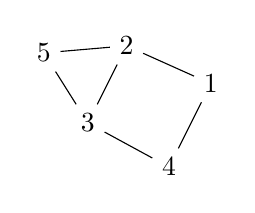
\begin{tikzpicture}
  \node (v0) at (1.15, 0.21) {1};
  \node (v1) at (0.08, 0.69) {2};
  \node (v2) at (-0.41, -0.29) {3};
  \node (v3) at (0.62, -0.85) {4};
  \node (v4) at (-0.97, 0.6) {5};
  \draw (v0) -- (v1);
  \draw (v0) -- (v3);
  \draw (v1) -- (v4);
  \draw (v1) -- (v2);
  \draw (v2) -- (v4);
  \draw (v2) -- (v3);
  \end{tikzpicture}
\end{example}

La clase de equivalencia de $2\rule[1mm]{4mm}{0.3mm}5$ es el conjunto:
$$S_{1} = \{2\rule[1mm]{4mm}{0.3mm}5, 5 \hdashrule[1mm]{4mm}{1pt}{1pt} 3\}$$
La clase de equivalencia de $1\hdashrule[1mm]{4mm}{1pt}{1pt} 4$ es el conjunto:
$$S_{2} = \{2 \hdashrule[1mm]{4mm}{1pt}{1pt} 1, 1\rule[1mm]{4mm}{0.3mm}4, 4\rule[1mm]{4mm}{0.3mm}3\}$$
La clase de equivalencia de $2\rule[1mm]{4mm}{0.3mm}3$ es el conjunto:
$$S_{3} = \{2\rule[1mm]{4mm}{0.3mm}3\}$$

Para saber si $\{2,3\}$ es un par de separación hay que encontrar una partición de $\{1, 2, 3\} = A \cup B$, $A \cap B = \{\emptyset\}$ tal que se cumpla que $|E_{1} = \bigcup_{i \in A} S_i| \geq 2$ y $ |E_{2}= \bigcup_{j \in B} S_j| \geq 2$.
En este caso $A = \{1, 3\}$, $B=\{2\}$ es una partición posible que buscamos y entonces $\{2, 3\}$ es un par de separación.\\

Ahora supongamos $\{a, b\}$ es un par de separación. Si $H=\{\{a, b\}, \emptyset\}$ y $S_{1},S_{2}, \ldots, S_{k}$ son las clases de separación del par $\{a, b\}$(las clases de equivalencia definidas por $H$).Sea $A, B$ la partición del conjunto $\{1,2,\ldots,k\}$ tal que $|E_1 = \bigcup_{i \in A} S_i| \geq 2$ y $ |E_{2}= \bigcup_{j \in B} S_j| \geq 2$. Si $H_{1} = (V(E_{1}), E_{1})$ y $H_{2} = (V(E_{2}), E_{2})$ entonces, $V(E_{1}) \cap V(E_{1}) = \{a, b\}$ donde la arista $a\rule[1mm]{4mm}{0.3mm} b$ es llamada arista virtual. Sea $G_{i} = H_{i} + \{a, b\}$ para $i \in \{1, 2\}$. Los $G_{i}$ son las gráficas de separación de $G$ en $\{a, b\}$. A la operación de reemplazar la gráfica $G$ por dos gráficas de separación llamaremos \textbf{separación} de $G$. Debe de haber muchas formas posibles de separar una gráfica, incluso con respecto a un par de separación fijo $\{a, b\}$. Una operación de separación se denota por $s\left(a, b, i\right)$; donde $i$ es un etiqueta que distingue esta operación de separación de otras separaciones. Una arista virtual $\left(a, b\right)$ asociada con la separación $s\left(a, b, i\right)$ se denotará por $\left(a, b, i\right)$. Si $G$ es biconexa, cualquier gráfica de separación de $G$ también es biconexa.

Si hay al menos dos clases de separación, entonces $\{a, b\}$ es una \textbf{par de separación} de $G$ a menos que $(i)$ haya exactamente dos clases de separación y una clase consta de una sola arista, o $(ii)$ hay exactamente tres clases, cada una de las cuales consta de una sola arista.

\paragraph{}
Si $G$ es una gráfica biconexa tal que ningún par $\{a, b\}$ es un par de separación de $G$, entonces $G$ es \textbf{triconexa}. 
\begin{figure}[H]
      \begin{subfigure}[b]{0.3\textwidth}
        \begin{minipage}{5cm}
            \centering% El subgrafo está centrado
            \begin{tikzpicture}
            \node (v0) at (1, 0) {};
            \node (v1) at (-1, 0) {};
            \node (v2) at (0.0, 1) {};
            \draw (v0) -- (v1);
            \draw (v0) -- (v2);
            \draw (v2) -- (v1);
            \end{tikzpicture}
        \end{minipage}
        \caption{Triangulos}
        \label{figura:Triangulos}
        \end{subfigure}
        \begin{subfigure}[b]{0.3\textwidth}
            \begin{minipage}{5cm}
                \centering% El subgrafo está centrado
                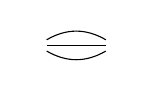
\begin{tikzpicture}
                \node(v0) at (0,0) {};
                \node(v1) at (1,0) {};
                \draw (v0) to (v1);
                \draw (v0) to[bend right] (v1);
                \draw (v1) to[bend right] (v0);
            \end{tikzpicture}
        \end{minipage}
        \caption{Enlaces}
        \label{figura:Enlaces}
        \end{subfigure}
        \begin{subfigure}[b]{0.3\textwidth}
            \begin{minipage}{5cm}
            \centering% El subgrafo está centrado
            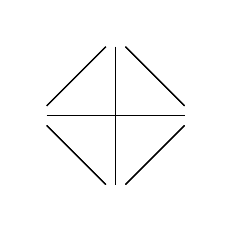
\begin{tikzpicture}
            \node (v0) at (1, 0.) {};
            \node (v1) at (-1, 0) {};
            \node (v2) at (0.0, -1) {};
            \node (v3) at (0.0, 1) {};
            \draw (v0) -- (v1);
            \draw (v0) -- (v2);
            \draw (v0) -- (v3);
            \draw (v1) -- (v0);
            \draw (v1) -- (v2);
            \draw (v1) -- (v3);
            \draw (v2) -- (v1);
            \draw (v2) -- (v0);
            \draw (v2) -- (v3);
            \draw (v3) -- (v2);
            \draw (v3) -- (v1);
            \draw (v3) -- (v0);
            \end{tikzpicture}
            \end{minipage}
            \caption{Poligonos}
            \label{figura:Poligonos}
            \end{subfigure}
    \caption{Ejemplos de componentes triconexas}
    \label{figura:triconexasEjemplo}
\end{figure}
		
\paragraph{}
Supongamos que separamos una gráfica $G$, las gráficas de separación se dividen, y así sucesivamente, hasta que no sean posibles más separaciones (cada gráfica restante es triconexa). Los gráficas construidas de esta manera se denominan \textbf{componentes de separación} de $G$. Los componentes de separación de una gráfica no son necesariamente únicos.
\begin{lemma}
Sea $G = \left(V, E \right)$ un gráfica con $\left| E \right| \geq 3$. Sea $G_{1}, G_{2}, \ldots G_{m}$ los componentes de separación de $G$. Entonces el número total de aristas en $G_{1}, G_{2}, \ldots , G_{m}$ está delimitado por $3\left| E \right| - 6$.
\label{lema:3.1}
\end{lemma}

\begin{proof}
 El lema se demuestra por inducción sobre el número de aristas de $G$. Si $G$ tiene $3$ aristas, el lema es inmediato, porque $G$ no se puede separar. Supongamos que el lema es cierto para gráficas con $n-1$ aristas y supongamos que $G$ tiene $n$ aristas. Si $G$ no puede ser dividido, el lema es verdadero para $G$. Supongamos, por otro lado, que $G$ se puede separar en $G^{'}$ y $G^{"}$, donde $G^{'}$ tiene $k + 1$ aristas y $G^{"}$ tiene $n - k + 1$ aristas tal que $2 \leq k \leq n - 2$. Por inducción, el número total de aristas en $G_{1}, G_{2}, \ldots G_{m}$ debe estar acotado por $3\left(k + 1\right) - 6 + 3\left(n - k + 1\right) - 6 = 3n - 6$. Así, por inducción, el lema 1 es cierto.
\end{proof}

\paragraph{}
Para obtener las componentes triconexas únicas, debemos volver a unir parcialmente los componentes de separación. Supongamos que $G_{1} = (V_{1},E_{1})$ y $G_{2}=(V_{2},E_{2})$ son dos componentes de separación, ambos con una arista virtual $\left(a, b, i\right)$. Sea
\begin{equation*}
G = \left(V_{1} \cup V_{2}, \left( E_{1} - \{\left(a, b, i\right)\}\right) \cup \left( E_{2} - \{\left(a, b, i\right)\}\right) \right)
\end{equation*}

\paragraph{}
Entonces a $G$ se le llama una \textbf{gráfica de unión} de $G_{1}$ y $G_{2}$; la operación de unión se denotará por $m\left(a, b, i \right)$. La unión es la inversa de la separación; si realizamos un suficiente número de uniones en los componentes divididos de una gráfica, recreamos la gráfica original.

\paragraph{}
Los componentes de separación de una gráfica son de tres tipos: 
\begin{enumerate}
\item enlaces triples de la forma $\left(\{a, b\}, \{\left(a, b\right),\left(a, b\right),\left(a, b\right)\} \right)$ \ref{figura:Enlaces}
\item triángulos de la forma $\left(\{a, b, c\}, \{\left(a, b\right),\left(a, c\right),\left(b, c\right)\}\right)$ \ref{figura:Triangulos}
\item gráficas triconexas \ref{figura:Poligonos}
\end{enumerate}
Sea $G$ una gráfica cuyos componentes de separación son un conjunto de enlaces triples $\mathscr{B}_{3}$, un conjunto de triángulos $\mathscr{F}$ y un conjunto de gráficas triconexas $\mathscr{C}$. Supongamos que los enlaces triples $\mathscr{B}_{3}$ se unen tanto como sea posible para dar un conjunto de enlaces $\mathscr{B}$ y que los triángulos $\mathscr{F}$ se unen tanto como sea posible para dar un conjunto de polígonos $\mathscr{P}$. Entonces el conjunto de gráficas $ \mathscr{B} \cup \mathscr{P} \cup \mathscr{C}$ es el conjunto de componentes triconexas de $G$. Si $G$ es una gráfica arbitraria, las componentes triconexas de las componentes biconexas de $G$ se les llama \textbf{componentes triconexas} de $G$.

\begin{lemma}
Las componentes triconexas de una gráfica $G$ son únicas
\label{lema:3.2}
\end{lemma}

\begin{proof}
Prueba. Ver \citep{mac-lane-1937}, \citep{jEdmonds} y \citep{tarjan-1972}.
\end{proof}

Tomemos como ejemplo el siguiente grafo para mostrar todo el procedimiento.
\begin{figure}[h]
\centering
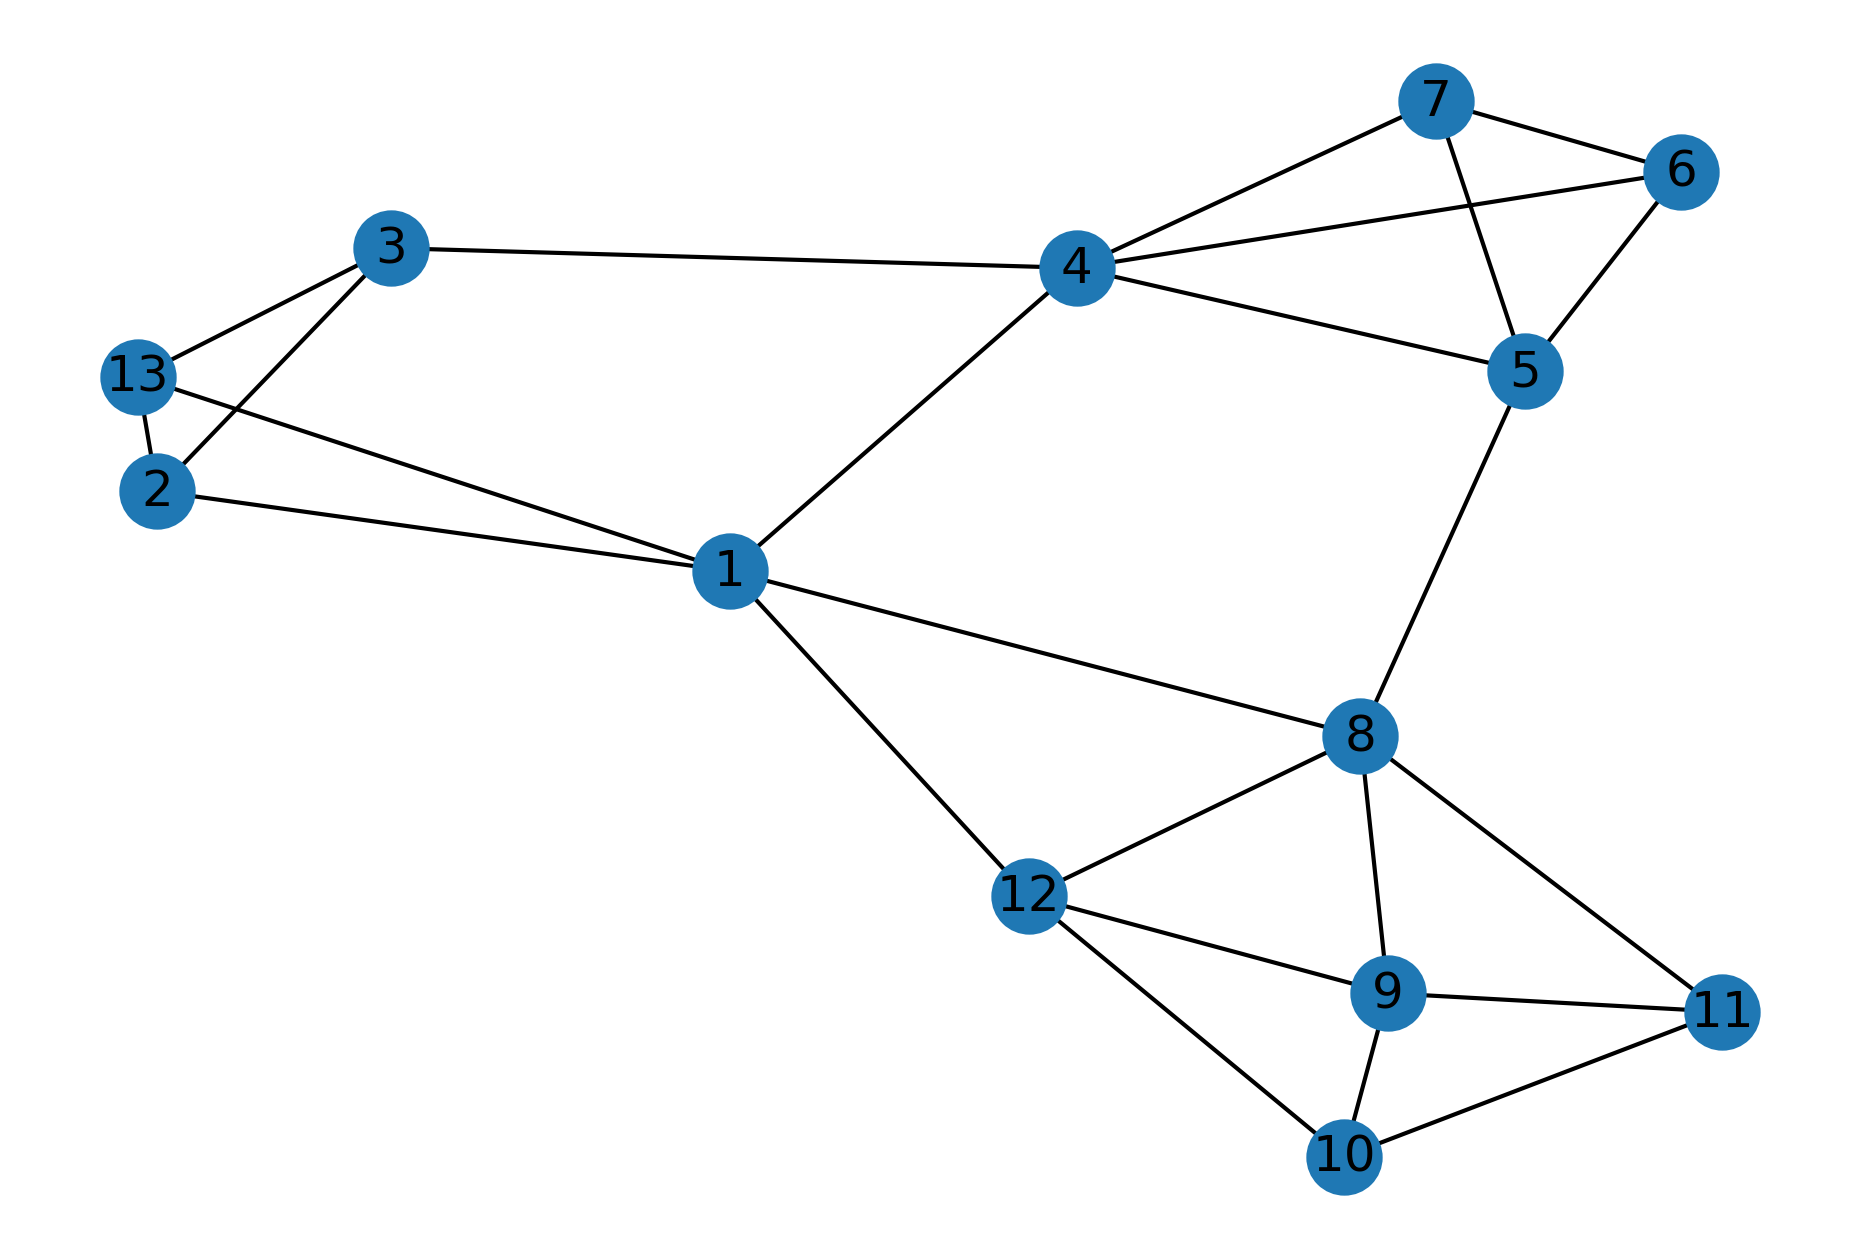
\includegraphics[width=10cm]{Figuras/plotgraph.png}
\caption{Una gráfica biconexa $G$ con pares de separación $(1, 4),(4, 5),(1, 8),(12, 8)$}
\label{figura:3.1}
\end{figure}

\begin{figure}[H]
      \begin{subfigure}[b]{0.3\textwidth}
        \begin{minipage}{7cm}
            \centering% El subgrafo está centrado
            \begin{tikzpicture}[scale=.4]
            \GraphInit[vstyle=Normal]
            %
            \tikzset{VertexStyle/.append style={minimum size=1pt, inner sep=1pt}}
            \Vertex[L=\hbox{$10$},x=2.4209cm,y=5.0cm]{v0}
            \Vertex[L=\hbox{$11$},x=5.0cm,y=2.5701cm]{v1}
            \Vertex[L=\hbox{$12$},x=0.0cm,y=2.4362cm]{v2}
            \Vertex[L=\hbox{$8$},x=2.574cm,y=0.0cm]{v3}
            \Vertex[L=\hbox{$9$},x=2.4254cm,y=2.4944cm]{v4}
            %
            \Edge[](v0)(v1)
            \Edge[](v0)(v2)
            \Edge[](v4)(v0)
            \Edge[](v3)(v1)
            \Edge[](v4)(v1)
            \Edge[](v4)(v2)
            \Edge[](v3)(v4)
            \tikzstyle{EdgeStyle}=[color=red]
            \tikzset{LabelStyle/.style = {fill=white, scale=.6}}
            \Edge[label=$A$](v3)(v2)
            %
            \end{tikzpicture}
        \end{minipage}
      \end{subfigure}
      \begin{subfigure}[b]{0.3\textwidth}
       \begin{minipage}{7cm}
            \centering% El subgrafo está centrado
            \begin{tikzpicture}[scale=.4]
            \GraphInit[vstyle=Normal]
            %
            \tikzset{VertexStyle/.append style={minimum size=1pt, inner sep=1pt}}
            \Vertex[L=\hbox{$12$},x=5.0cm,y=5.0cm]{v0}
            \Vertex[L=\hbox{$8$},x=0.0cm,y=0.0cm]{v1}
            %
            \Edge[](v1)(v0)
            \tikzstyle{EdgeStyle}=[color=red]
            \tikzset{LabelStyle/.style = {fill=white, scale=.6}}
            \Edge[label=$A$, style={bend left}](v1)(v0)
            \Edge[label=$B$, style={bend right}](v1)(v0)
            %
            \end{tikzpicture}
       \end{minipage}
      \end{subfigure}
      \begin{subfigure}[b]{0.3\textwidth}
       \begin{minipage}{7cm}
            \centering% El subgrafo está centrado
            \begin{tikzpicture}[scale=.4]
            \GraphInit[vstyle=Normal]
            %
            \tikzset{VertexStyle/.append style={minimum size=1pt, inner sep=1pt}}
            \Vertex[L=\hbox{$12$},x=5.0cm,y=2.1281cm]{v0}
            \Vertex[L=\hbox{$1$},x=0.0cm,y=0.0cm]{v1}
            \Vertex[L=\hbox{$8$},x=0.51cm,y=5.0cm]{v2}
            %
            \Edge[](v1)(v0)
            \tikzstyle{EdgeStyle}=[color=red]
            \tikzset{LabelStyle/.style = {fill=white, scale=.6}}
            \Edge[label=$C$](v1)(v2)
            \Edge[label=$B$](v2)(v0)
            %
            \end{tikzpicture}
       \end{minipage}
      \end{subfigure}
      \begin{subfigure}[b]{0.3\textwidth}
       \begin{minipage}{7cm}
            \centering% El subgrafo está centrado
            \begin{tikzpicture}[scale=.4]
            \GraphInit[vstyle=Normal]
            %
            \tikzset{VertexStyle/.append style={minimum size=1pt, inner sep=1pt}}
            \Vertex[L=\hbox{$1$},x=0.0cm,y=5.0cm]{v0}
            \Vertex[L=\hbox{$8$},x=5.0cm,y=0.0cm]{v1}
            %
            \Edge[](v0)(v1)
            \tikzstyle{EdgeStyle}=[color=red]
            \tikzset{LabelStyle/.style = {fill=white, scale=.6}}
            \Edge[label=$C$, style={bend left}](v1)(v0)
            \Edge[label=$D$, style={bend right}](v1)(v0)
            %
            \end{tikzpicture}
       \end{minipage}
      \end{subfigure}
      \begin{subfigure}[b]{0.3\textwidth}
       \begin{minipage}{7cm}
            \centering% El subgrafo está centrado
            \begin{tikzpicture}[scale=.4]
            \GraphInit[vstyle=Normal]
            %
            \tikzset{VertexStyle/.append style={minimum size=1pt, inner sep=1pt}}
            \Vertex[L=\hbox{$1$},x=0.0cm,y=5.0cm]{v0}
            \Vertex[L=\hbox{$5$},x=1.4425cm,y=0.0cm]{v1}
            \Vertex[L=\hbox{$8$},x=5.0cm,y=3.8666cm]{v2}
            %
            \Edge[](v1)(v2)
            \tikzstyle{EdgeStyle}=[color=red]
            \tikzset{LabelStyle/.style = {fill=white, scale=.6}}
            \Edge[label=$E$](v0)(v1)
            \Edge[label=$D$](v0)(v2)
            
            %
            \end{tikzpicture}
       \end{minipage}
      \end{subfigure}
      \begin{subfigure}[b]{0.3\textwidth}
       \begin{minipage}{7cm}
            \begin{tikzpicture}[scale=.4]
            \GraphInit[vstyle=Normal]
            %
            \tikzset{VertexStyle/.append style={minimum size=1pt, inner sep=1pt}}
            \Vertex[L=\hbox{$4$},x=2.2676cm,y=0.0cm]{v0}
            \Vertex[L=\hbox{$5$},x=0.0cm,y=2.8922cm]{v1}
            \Vertex[L=\hbox{$6$},x=2.7386cm,y=5.0cm]{v2}
            \Vertex[L=\hbox{$7$},x=5.0cm,y=2.1171cm]{v3}
            %
            \Edge[](v0)(v2)
            \Edge[](v0)(v3)
            \Edge[](v1)(v2)
            \Edge[](v1)(v3)
            \Edge[](v2)(v3)
            \tikzstyle{EdgeStyle}=[color=red]
            \tikzset{LabelStyle/.style = {fill=white, scale=.6}}
            \Edge[label=$F$](v0)(v1)
            %
            \end{tikzpicture}
       \end{minipage}
      \end{subfigure}
      \begin{subfigure}[b]{0.3\textwidth}
       \begin{minipage}{7cm}
            \centering% El subgrafo está centrado
            \begin{tikzpicture}[scale=.4]
            \GraphInit[vstyle=Normal]
            %
            \tikzset{VertexStyle/.append style={minimum size=1pt, inner sep=1pt}}
            \Vertex[L=\hbox{$4$},x=0.0cm,y=0.0cm]{v0}
            \Vertex[L=\hbox{$5$},x=5.0cm,y=5.0cm]{v1}
            %
            \Edge[](v0)(v1)
            \tikzstyle{EdgeStyle}=[color=red]
            \tikzset{LabelStyle/.style = {fill=white, scale=.6}}
            \Edge[label=$F$, style={bend left}](v0)(v1)
            \Edge[label=$G$, style={bend right}](v0)(v1)
            %
            \end{tikzpicture}
       \end{minipage}
      \end{subfigure}
      \begin{subfigure}[b]{0.3\textwidth}
       \begin{minipage}{7cm}
            \centering% El subgrafo está centrado
            \begin{tikzpicture}[scale=.4]
            \GraphInit[vstyle=Normal]
            %
            \tikzset{VertexStyle/.append style={minimum size=1pt, inner sep=1pt}}
            \Vertex[L=\hbox{$1$},x=0.0cm,y=5.0cm]{v0}
            \Vertex[L=\hbox{$4$},x=2.0511cm,y=0.0cm]{v1}
            \Vertex[L=\hbox{$5$},x=5.0cm,y=4.3924cm]{v2}
            %
            \tikzstyle{EdgeStyle}=[color=red]
            \tikzset{LabelStyle/.style = {fill=white, scale=.6}}
            \Edge[label=$H$](v0)(v1)
            \Edge[label=$E$](v0)(v2)
            \Edge[label=$G$](v1)(v2)
            %
            \end{tikzpicture}
       \end{minipage}
      \end{subfigure}
      \begin{subfigure}[b]{0.3\textwidth}
       \begin{minipage}{7cm}
            \centering% El subgrafo está centrado
            \begin{tikzpicture}[scale=.4]
            \GraphInit[vstyle=Normal]
            %
            \tikzset{VertexStyle/.append style={minimum size=1pt, inner sep=1pt}}
            \Vertex[L=\hbox{$1$},x=5.0cm,y=5.0cm]{v0}
            \Vertex[L=\hbox{$4$},x=0.0cm,y=0.0cm]{v1}
            %
            \Edge[](v0)(v1)
            \tikzstyle{EdgeStyle}=[color=red]
            \tikzset{LabelStyle/.style = {fill=white, scale=.6}}
            \Edge[label=$I$, style={bend left}](v0)(v1)
            \Edge[label=$H$, style={bend right}](v0)(v1)
            %
            \end{tikzpicture}
       \end{minipage}
      \end{subfigure}
      \begin{subfigure}[b]{0.5\textwidth}
       \begin{minipage}{7cm}
            \centering% El subgrafo está centrado
            \begin{tikzpicture}[scale=.4]
            \GraphInit[vstyle=Normal]
            %
            \tikzset{VertexStyle/.append style={minimum size=1pt, inner sep=1pt}}
            \Vertex[L=\hbox{$1$},x=5.0cm,y=0.202cm]{v0}
            \Vertex[L=\hbox{$3$},x=0.0cm,y=0.0cm]{v1}
            \Vertex[L=\hbox{$4$},x=2.3629cm,y=5.0cm]{v2}
            %
            \Edge[](v1)(v2)
            \tikzstyle{EdgeStyle}=[color=red]
            \tikzset{LabelStyle/.style = {fill=white, scale=.6}}
            \Edge[label=$J$](v0)(v1)
            \Edge[label=$I$](v0)(v2)
            
            %
            \end{tikzpicture}
       \end{minipage}
      \end{subfigure}
      \begin{subfigure}[b]{0.5\textwidth}
       \begin{minipage}{7cm}
            \centering% El subgrafo está centrado
            \begin{tikzpicture}[scale=.4]
            \GraphInit[vstyle=Normal]
            %
            \tikzset{VertexStyle/.append style={minimum size=1pt, inner sep=1pt}}
            \Vertex[L=\hbox{$13$},x=0.0cm,y=1.6413cm]{v0}
            \Vertex[L=\hbox{$1$},x=5.0cm,y=3.3643cm]{v1}
            \Vertex[L=\hbox{$2$},x=3.4414cm,y=0.0cm]{v2}
            \Vertex[L=\hbox{$3$},x=1.556cm,y=5.0cm]{v3}
            %
            \Edge[](v1)(v0)
            \Edge[](v2)(v0)
            \Edge[](v3)(v0)
            \Edge[](v1)(v2)
            \Edge[](v2)(v3)
            \tikzstyle{EdgeStyle}=[color=red]
            \tikzset{LabelStyle/.style = {fill=white, scale=.6}}
            \Edge[label=$J$](v1)(v3)
            %
            \end{tikzpicture}
       \end{minipage}
      \end{subfigure}
\caption{Componentes de separación de $G$ las componentes triconexas se forma al unir los triangulos $(1, 4, 5)$ y $(1, 5, 8)$}
\label{figura:3.2}
\end{figure}

\paragraph{}
Los algoritmos de gráficas requieren una forma sistemática de explorar una gráfica. En el articulo \citep{hopcroft1973} se utiliza un método llamado \textbf{búsqueda en profundidad}. Para llevar a cabo una búsqueda en profundidad en $G$, se comienza desde algún vértice $s$ y se elije una arista que vaya desde $s$ a otro vértice $w$ en el gráfica, después se marca el vértice $s$ como visitado y se elige ahora $w$ como punto de partida ahora vamos a elegir alguna arista que conecta $w$ cuyo vértice que la conecta a $w$ aun no haya sido visitado si cumple esto elegimos esta arista y marcamos a $w$ como visitado y continuamos así hasta que ya no haya vértices a los cuales visitar. Si $G$ es conexa, cada arista se recorre exactamente una vez*.

\paragraph{}
Si $G$ no es dirigida, una búsqueda sobre $G$ impone una dirección en cada arista de $G$ dada por la dirección en la que se recorre la arista durante la búsqueda. Así la búsqueda convierte $G$ en una gráfica dirigida $G^{'}$.

\begin{lemma}
Sea $P$ la gráfica dirigida generada por una búsqueda en profundidad de una gráfica no dirigida conexa $G$. Entonces $P$ es un árbol de recorrido.
\label{lema:3.3}
\end{lemma}

\begin{proof}
Véase \citep{4569669}.
\end{proof}

\paragraph{}
La búsqueda primero en profundidad es importante porque la estructura de los caminos en un árbol es muy simple. Para implementar una búsqueda en profundidad de una gráfica, usamos un procedimiento recursivo simple que mantiene una pila de los viejos vértices con posiblemente aristas inexploradas. Para representar un gráfica, se utiliza un conjunto de \textbf{listas de adyacencia}, uno para cada vértice. Si $v$ es un vértice la lista de adyacencia $A\left(v\right)$ contiene todos los $w$ tales que $\left(v, w\right)$ es una arista de $G$. Estas listas juntas comprenden una \textbf{estructura de adyacencia} para $G$. Si $G$ no es dirigida, cada arista $\left(v, w\right)$ se representa dos veces, una en $A\left(v\right)$ y otra en $A\left(w\right)$. 

\paragraph{}
\ref{alg:busqueda en profundidad} muestra un procedimiento recursivo para realizar una búsqueda en profundidad. La búsqueda exacta depende del orden de los aristas en las listas de adyacencia. Los números de procedimiento de los vértices del $1$ al $V$ en el orden en que se alcanzan durante el búsqueda, además de identificar arcos y ramas de el árboles de recorrido y aristas de retroceso que nos ayudan mas adelante. La referencia \citep{4569669} da una prueba que el procedimiento es correcto y requiere tiempo $\Theta \left(V + E\right)$ para ejecutarse. Los vértices están numerados de modo que $NUMBER\left(v\right) \le NUMBER\left(w\right)$ si $ v \overset{\ast}{\rightarrow} w$ en el árbol generado.


\begin{algorithm}[!ht]
\DontPrintSemicolon
\tcp{a: declaración vacía}\;
\For{cada $w$ in $A\left(v\right)$}{
 	\If{$NUMBER(w)$ = 0}{
 		marcamos a $(v, w)$ como una rama de el árbol\;
 		$DFS(w, v)$\;
 		\tcp{b: declaración vacía}\;
 	}
 	\ElseIf{($NUMBER(w) < NUMBER(v))$ and (($w \neq u$) or $\neg FLAG(v)$)}{
        marcamos $(v, w)$ como arista de retroceso\;
        \tcp{b: declaración vacía}\;
 	}
 	\If{w=u}{
        $FLAG(v) = false$\:
 	}
}
\DontPrintSemicolon
$n=0$\;
\For{$i=1$ to $V$:}{
    $NUMBER(i) = 0$\;
    $FLAG(i) = True$\;
    }
$DFS(1, 0)$\;
\caption{DFS($v, u$)}\label{alg:busqueda en profundidad}
\end{algorithm}

\paragraph{}
Las declaraciones a, b, c, se reemplazarán cuando se use DFS para calcular otra información sobre el gráfica. En \ref{figura:3.3} representa el árbol formado aplicando DFS y también las aristas de backtracking $a \hookrightarrow b$ que son necesarias para nuestro algoritmo. En rojo están coloreadas las aristas de DFS y en azul el Backtracking de estas aristas y identificar los valores de lowpt1 y lowpt2.

\begin{figure}[H]
\centering
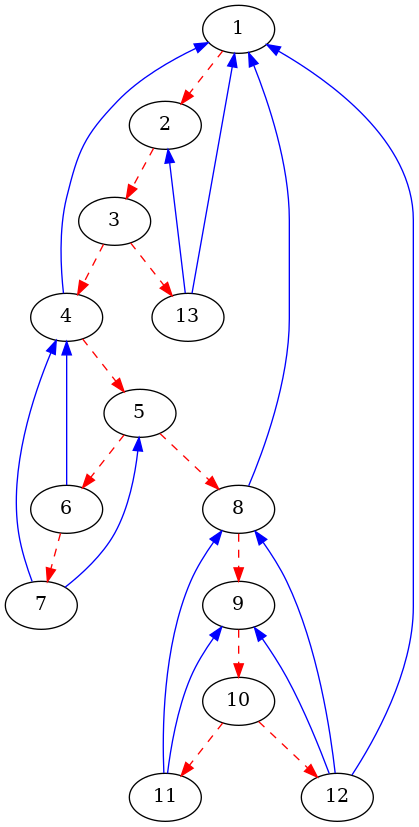
\includegraphics[width=6cm]{Figuras/G2.png}
\caption{Árbol de recorrido generado por la búsqueda primero en profundidad de $G$ en \ref{figura:3.1}}
\label{figura:3.3}
\end{figure}

\subsection{La idea de el algoritmo de triconectividad}

\paragraph{}
Esta sección esboza las ideas detrás del algoritmo de triconectividad. Las secciones posteriores desarrollan los componentes detallados. El algoritmo se basa en una idea de Auslander, Parter y Goldstein (\citep{auslander-1961}, \citep{goldstein1963efficient}) para probar la planaridad de los gráficas. La idea de Auslander, Parter y Goldstein da lugar a un algoritmo de tiempo $\Theta\left(V\right)$ para probar la planaridad, si la búsqueda primero en profundidad se utiliza para ordenar los cálculos de (\citep{efalgm}, \citep{ept}). La misma idea da un tiempo $\Theta\left(V + E\right)$ para el algoritmo de encontrar componentes triconexas.

\paragraph{}
Sea $G$ una gráfica biconexo arbitrario. Supongamos que un ciclo $c$ se encuentra en $G$. Cuando se elimina el ciclo de $G$ quedan ciertas piezas conectadas; a estos se les llama \textbf{segmentos}. Auslander y Parter \citep{auslander-1961} demuestran que $G$ es plano si y solo si
\begin{enumerate}
\item Cualquier subgráfica de $G$ que consta de $c$ más un solo segmento es plano.
\item Los segmentos pueden combinarse consistentemente para dar una incrustación plana de todo la gráfica.
\end{enumerate}
Se puede desarrollar un algoritmo de planaridad eficiente a partir de este resultado(\citep{efalgm}, \citep{ept}). A resultado similar se cumple para los pares de separación de $G$, es decir, el siguiente lema.

\begin{lemma}
Sea $G$ una gráfica biconexa y sea $c$ un ciclo en $G$. Sea $S_{1}, \ldots, S_{m}$ las subgráficas de $G \rule[1mm]{.1cm}{0.4pt} c$ tales que $e_{1}$ y $e_{2}$ son aristas de $S_{i}$ si y sólo si algún camino $p$ en $G$ contiene tanto $e_{1}$ como $e_{2}$ y ningún vértice de $c$ se encuentra entre $e_{1}$ y $e_{2}$ en $p$. Los segmentos $S_{i}$ y el ciclo $c$ particionan las aristas de $G$. Sea $\{a, b\}$ un par de separación de $G$ ,entonces se cumplen las siguientes conclusiones.
\begin{enumerate}
\item Tanto $a$ como $b$ se encuentran en $c$, o bien $a$ y $b$ se encuentran ambos en algún segmento $S_{i}$.
\item Supongamos que tanto $a$ como $b$ están en $c$. Sean $p_{1}$ y $p_{2}$ los dos caminos que componen $c$ los cuales unen $a$ y $b$. Entonces o
\begin{enumerate}
\item Algún segmento $S_{i}$ con al menos dos aristas tiene solo a $a$ y $b$ en común con $c$, y algún vértice $v$ no está en $S_{i}$ ($\{a, b\}$ se le dice par de separación de ''tipo 1''), o
\item Ningún segmento contiene un vértice $v \neq a, b$ en $p_{1}$ y un vértice $w \neq a, b$ en $p_{2}$, $p_{1}$ y $p_{2}$ contienen cada uno un vértice además de $a$ y $b$ ($\{a, b\}$ se le dice par de separación de ''tipo 2'').
\end{enumerate}
\item A la inversa, cualquier par $\{a, b\}$ que satisfaga (a) o (b) es un par de separación.
\end{enumerate}
\label{lema:3.4}
\end{lemma}

\paragraph{}

El lema \ref{lema:3.4} da lugar a un algoritmo recursivo eficiente para encontrar componentes de separación. Encontramos un ciclo en $G$ y determinamos los segmentos formados cuando es eliminado. Probamos cada segmento en busca de pares de separación aplicando el algoritmo recursivamente y probamos el ciclo para pares de separación verificando los criterios en lema \ref{lema:3.4}. La aplicación recursiva del algoritmo requiere encontrar ciclos en subgráficas de $G$ formados por la combinación de un segmento $S_{i}$ y el ciclo inicial $c$.

\paragraph{}
Podemos hacer que este algoritmo sea muy eficiente ordenando los cálculos usando búsqueda en profundidad. Cada llamada recursiva en el algoritmo requiere que encontremos un ciclo en la parte de la gráfica que se va a probar para los pares de separación. Este ciclo constará de un camino simple de aristas las cuales no están en ciclos previamente encontrados más un camino simple de aristas en ciclos no encontrados. Usamos la búsqueda primero en profundidad para separar la gráfica en caminos simples que pueden ensamblarse en estos ciclos. El primer ciclo $c$ consistirá en una secuencia de aristas del árbol seguidos por una arista en $P$, el árbol formado a partir de $G$ por búsqueda primero en profundidad. La numeración de vértices es tal que los vértices están ordenados por número a lo largo del ciclo. Cada segmento consistirá en una sola arista $\left(v, w\right)$ o en una arista $\left(v, w\right)$ de el árbol más un subárbol con raíz $w$, además todas las ramas que salen del subárbol. La búsqueda explora los segmentos en orden decreciente de $v$ y divide cada uno en caminos simples que consisten en una secuencia de ramas de el árbol seguido por una vértice.

\paragraph{}
Encontrar caminos en realidad requiere dos búsquedas porque la búsqueda de caminos debe llevarse a cabo en un orden especial para tener éxito, y ciertos cálculos preliminares son necesarios. La sección sobre cómo encontrar pares de separación describe la proceso de búsqueda de caminos en detalle e incluye una versión del lema \ref{lema:3.4} que caracteriza pares de separación en términos de los caminos generados. La sección de encontrar componentes de separación indica cómo se pueden usar estos resultados para determinar los componentes de separación de una gráfica biconexa en tiempo $\Theta \left(V + E\right)$.

\paragraph{}
Para determinar las componentes triconexas de una gráfica arbitrarias, encontramos las componentes biconexas de la gráfica usando el algoritmo $\Theta \left(V + E\right)$ descrito en \citep{4569669} y \citep{efalgm}. A continuación, los componentes de separación de cada componente biconexa se encuentran utilizando el algoritmo descrito anteriormente y presentado en detalle en el siguiente dos secciones. Esto nos da los componentes de separación de toda la gráfica. El tamaño total de las componentes de separación es $\Theta \left(V + E\right)$, por el lema \ref{lema:3.1}. A continuación identificamos el conjunto de enlaces triples $\mathscr{B}_{3}$ y el conjunto de triángulos $\mathscr{T}$. Para cada uno de estos dos conjuntos, construimos una gráfica auxiliar $S$ cuyos vértices son los elementos del conjunto; dos componentes de separación están unidos por una arista en una gráfica auxiliar si tienen un arista virtual común. Los componentes conectados de $S\left(\mathscr{B}_{3}\right)$ y $S\left(\mathscr{T}\right)$ corresponden a los enlaces y polígonos que son componentes triconexas de $G$. Encontrar estos enlaces y polígonos requiere tiempo $\Theta \left(V + E\right)$. A continuación se muestra un esquema de todo el algoritmo de acuerdo a \citep{Gutwenger2000ALT}.

\section{El algoritmo para encontrar componentes triconexas}

\begin{algorithm}[!ht]
\DontPrintSemicolon
 A: Encontramos las componentes biconexas de $G$;\;
 \For{cada componente biconexa $\mathcal{C}$ de $G$}{
 	B: encontrar los componentes de separación de $C$;\;
 	C: combinar los triangulos en poligonos al encontrar las componentes conexas correspondientes a las gráficas auxiliares;\;
 } 
\caption{TRICONNECTIVITY($G$)}\label{alg:triconexidad}
\end{algorithm}

\paragraph{}
Los pasos A y C requieren tiempo $\Theta \left(V + E\right)$ si se implementan correctamente. La implementación del paso A se describe en \citep{4569669}. El paso difícil es el paso B, cuya implementación se describe en el siguientes dos secciones. Con base en los resultados de estas secciones, toda el algoritmo de triconectividad esta acotado por $\Theta  \left(V + E\right)$.

\subsection{Encontrando pares de separación}

\paragraph{}
Sea $G = \left(\mathscr{V}, \mathscr{E}\right)$ una gráfica biconexa con vértices $V$ y aristas $E$. El problema principal al separar $G$ en sus componentes de separación radica en encontrar sus pares de separación. Esta sección da un criterio simple, basado en la búsqueda primero en profundidad, para identificar los pares de separación de una gráfica. Se deben realizar dos búsquedas en profundidad y algunos cálculos auxiliares. Estos cálculos forman la primera parte del algoritmo de componentes separación y se describen a continuación. Las definiciones de las cantidades lowpt1, ND, etc., utilizadas en el el esquema se dará posteriormente.

\paragraph{Paso 1}
Realice una búsqueda primero en profundidad en el gráfica $G$, convirtiendo $G$ en un árbol $P$. Numeramos los vértices de $G$ en el orden en que se alcanzan durante la búsqueda. Calculamos lowpt1$\left(v\right)$, lowpt2$\left(v\right)$, nd$\left(v\right)$ y padre$\left(v\right)$ para cada vértice $v$ en $P$.

\paragraph{Paso 2}
Construimos una estructura de adyacencia aceptable $A$ para $P$ ordenando las aristas en la estructura de adyacencia de acuerdo con los valores de lowpt1 y lowpt2.

\paragraph{Paso 3}
Realizar una búsqueda en profundidad sobre $P$ utilizando la estructura de adyacencia $A$. Volvemos a numerar los vértices de $A$ desde $V$ a $1$ en el orden en que se examinaron por última vez durante la búsqueda. Particionamos las aristas en caminos simples disjuntos. Recalculamos lowpt1$\left(v\right)$ y lowpt2$\left(v\right)$ utilizando los nuevos números de los vértices. Calculamos A1$\left(v\right)$, deg$\left(v\right)$, y highpt$\left(v\right)$ para cada vértice $v$.

\paragraph{}
Los detalles de estos cálculos aparecen a continuación. Desde los pasos 1, 2 y 3, obtenemos suficiente información para determinar rápidamente los pares de separación de $G$. lema \ref{lema:3.13} da una condición para este propósito.

\paragraph{}
Supongamos que $G$ se explora primero en profundidad, dando un árbol $P$. Sean los vértices de $P$ numerados desde $1$ a $V$ de modo que $v \overset{\ast}{\rightarrow} w$ en $P$ implica que $v \le w$, si identificamos los vértices por su número. Para cualquier vértice $v$ en $P$, sea padre$\left(v\right)$ el padre de $v$ en el árbol de $P$. Sea ND$\left(v\right)$ el número de descendientes de $v$. Sea lowpt1$\left(v\right) = min\left(\{v\} \cup \{w | v \overset{\ast}{\rightarrow} \rule[1mm]{.1cm}{0.4pt} \rightarrow w\}\right)$. Es decir, lowpt1$\left(v\right)$ es el vértice más bajo alcanzable desde $v$ atravesando cero o más ramas de árbol en $P$ seguido de en la mayoría una arista. Sea lowpt2$\left(v\right) = min\left[\{v\} \cup \left(\{w | v \overset{\ast}{\rightarrow} \rule[1mm]{.1cm}{0.4pt} \rightarrow w\} - \{lowpt1 \left(v\right)\}\right)\right]$. Es decir, lowpt2$\left(v\right)$ es el segundo vértice más bajo alcanzable desde $v$ atravesando cero o más ramas de el árbol seguidas por una arista de $P$ como máximo, a menos que lowpt1$\left(v\right) = v$. En este caso, lowpt2$\left(v\right) = v$.

\begin{lemma}
lowpt1$\left(v\right)$ $  \overset{\ast}{\rightarrow} v$ y lowpt2$\left(v\right) \overset{\ast}{\rightarrow}v$ en $P$.
\label{lema:3.5}
\end{lemma}

\begin{proof}
lowpt1$\left(v\right) \leq v$ por definición. Si lowpt1$\left(v\right) = v$, el resultado es inmediato. Si lowpt1$\left(v\right) \le v$, hay una rama $u \rule[1mm]{.1cm}{0.4pt} \rightarrow $lowpt1$(v)$ tal que $v \overset{\ast}{\rightarrow} u$. Como $u \rule[1mm]{.1cm}{0.4pt} \rightarrow $lowpt1$(v)$ es una rama, lowpt1$\left(v\right) \overset{\ast}{\rightarrow} u$. Como $P$ es un árbol, $v \overset{\ast}{\rightarrow} u$ y\\ lowpt1$\left(v\right) \overset{\ast}{\rightarrow} u$, ya sea que $v \overset{\ast}{\rightarrow} $lowpt1$\left(v\right)$ o lowpt1$\left(v\right) \overset{\ast}{\rightarrow} v$. Pero lowpt1$\left(v\right) \le v$. Así debe ser el caso que lowpt1$\left(v\right) \overset{\ast}{\rightarrow} v \overset{\ast}{\rightarrow} u$, y el lema se cumple para lowpt1$\left(v\right)$. La demostración es la misma para lowpt2$\left(v\right)$.
\end{proof}

\begin{lemma}
Supongamos que lowpt1$\left(v\right)$ y lowpt2$\left(v\right)$ se definen en relación con alguna numeración para la cual $v \overset{\ast}{\rightarrow} w$ en $P$ implica NUMERO$\left(v\right) < $ NUMERO$\left(v\right)$. Entonces lowpt1$\left(v\right)$ y lowpt2$\left(v\right)$ identifican vértices únicos independientemente de la numeración usada.
\label{lema:3.6}
\end{lemma}

\begin{proof}
lowpt1$\left(v\right)$ siempre identifica a un ancestro del vértice $v$. Además,\\ lowpt1$\left(v\right)$ es el ancestro con el número más bajo de $v$ con cierta propiedad relativa al árbol $P$. Dado que el orden de los ancestros de $v$ corresponde al orden de sus números, lowpt1$\left(v\right)$ identifica a un único vértice independiente de la numeración, es decir, el primer ancestro de $v$ a lo largo de el camino  $1 \overset{\ast}{\rightarrow} v$ tiene la propiedad deseada(Cualquier numeración satisfactoria asigna $1$ a la raíz de $P$.) La prueba es la misma para lowpt2$\left(v\right)$.
\end{proof}

\paragraph{}
Los valores lowpt de un vértice $v$ dependen solo de los valores lowpt de los hijos de $v$ y en las ramas que salen de $v$; es fácil ver que si los vértices se identifican por número, entonces

\begin{equation*}
lowpt1\left(v\right)= min\left(\{v\} \cup \{lowpt1\left(w\right)| v \rightarrow w\} U \{w| v \rule[1mm]{.1cm}{0.4pt} \rightarrow w\}\right)
\end{equation*}
y
\begin{equation*}
\begin{split}
lowpt2\left(v\right) &=  min(\{v\} \cup ((\{lowpt1\left(w\right)| v \rightarrow w\}\\ 
				   & 	\hspace{0.8cm} \cup \{lowpt2\left(w\right)| v \rightarrow w\} \\
				   &	\hspace{0.8cm} \cup \{w | v \rule[1mm]{.1cm}{0.4pt} \rightarrow  w\}) \newline - \{lowpt1v\})).
\end{split}
\end{equation*}

En el caso de la gráfica anterior los valores de lowpt1 y lowpt2 son los siguientes:\\
\begin{center}
\begin{tabular}{lll}
\toprule
vértice & lowpt1 & lowpt2 \\
\midrule
      1 &      1 &      1 \\
      2 &      1 &      2 \\
      3 &      1 &      2 \\
      4 &      1 &      4 \\
      5 &      1 &      4 \\
      6 &      4 &      5 \\
      7 &      4 &      5 \\
      8 &      1 &      8 \\
      9 &      1 &      8 \\
     10 &      1 &      8 \\
     11 &      8 &      9 \\
     12 &      1 &      8 \\
     13 &      1 &      2 \\
\bottomrule
\end{tabular}
\end{center}

\paragraph{}
También tenemos nd$\left(v\right)= 1 + \sum_{v \rightarrow w} $ ND$\left(w\right)$. Podemos calcular los valores de lowpt, nd y padre para todos los vértices en tiempo $\Theta\left(V + E\right)$ insertando las siguientes declaraciones para las declaraciones a, b, c en DFS. La numeración de los vértices en el orden en que se alcanzan durante la búsqueda garantiza claramente que $v \overset{\ast}{\rightarrow} w$ implica $v \le w$.


\begin{algorithm}[!ht]
\DontPrintSemicolon
a: lowpt1$\left(v\right)$ = lowpt2$\left(v\right)$ = NUMERO$\left(v\right)$; \;
\hspace{0.4cm} ND$\left(v\right)$ = 1 \;
b: \If{lowpt1$\left(w\right) < $ lowpt1$\left(v\right)$}{
	\hspace{0.4cm} lowpt2$\left(v\right) = min\{$lowpt2$\left(v\right), $lowpt2$\left(w\right)\}$\;
	\hspace{0.4cm} lowpt1$\left(v\right) = $ lowpt1$\left(w\right)$\;
	}
\hspace{0.4cm} \ElseIf{lowpt1$\left(w\right) = $ lowpt1$\left(v\right)$}{
   	\hspace{0.4cm} lowpt2$\left(v\right) = min\{$lowpt2$\left(v\right), $lowpt2$\left(w\right)\}$
   }
\hspace{0.4cm} \Else{
   	\hspace{0.4cm} lowpt2$\left(v\right) = \{$ lowpt2$\left(v\right), $lowpt1$\left(w\right)\}$
   }
\hspace{0.4cm} ND$\left(v\right) = $ ND$\left(v\right) + $ND$\left(w\right)$\;
\hspace{0.4cm} FATHER$\left(w\right) = v$\;
c: \If{NUMERO$\left(w\right) < $ lowpt1$\left(v\right)$}{
	\hspace{0.4cm} lowpt2$\left(v\right) = $ lowpt1$\left(v\right)$\;
	\hspace{0.4cm} lowpt1$\left(v\right) = $ NUMERO$\left(w\right)$\;
	}
\hspace{0.4cm} \ElseIf{NUMERO$\left(w\right) = $lowpt1$\left(v\right)$}{
   	\hspace{0.4cm} lowpt2$\left(v\right) = min\{$lowpt2$\left(v\right), $NUMERO$\left(w\right)\}$
   }
\caption{adiciones a DFS($G$)}\label{alg:adicionales a DFS}
\end{algorithm}

\paragraph{}
Verificamos que DFS modificado anteriormente calculará lowpt1, lowpt2, ND y FATHER correctamente en tiempo $\Theta\left(V + E\right)$. (Ver \citep{ept}, \citep{tarjan-1972}.) lowpt1 puede usarse para probar la biconectividad de $G$, como se describe en \citep{4569669}. El siguiente lema es importante.

\begin{lemma}
Si $G$ es biconexa y $v \rightarrow w$, lowpt1$\left(w\right) \le v$ a menos que $v=1$, en cuyo caso lowpt1$\left(w\right) = v = 1$. Además, lowpt1$\left(1\right) = 1$.
\label{lema:3.7}
\end{lemma}

\begin{proof}
Véase [5].
\end{proof}

\paragraph{}
Sea $\phi$ el mapeo de las aristas de $P$ en $\{1, 2, \ldots, 2V + 1\}$ definido por:
\begin{equation*}
\phi(x) =
\begin{cases}
3lowpt1(w) & \text{si $e = v \rightarrow w$ y lowpt$2(w) < v$}\\
3w + 1 & \text{si $e = v \hookrightarrow w$}\\
3lowpt1(w) + 2 & \text{if $e = v \rightarrow w$ y lowpt$2(w) \geq v$}
\end{cases}
\end{equation*}
Sea $A$ una estructura de adyacencia para $P$. $A$ se le dice aceptable si las aristas $e$ en cada lista de adyacencia de $A$ se ordena de forma creciente de acuerdo a $\phi(e)$.

Lo cual da el siguiente resultado de \ref{figura:3.1} en forma de mapeo a cada vértice $1, 2,\ldots, 13$ los vértices adyacentes ordenados de acuerdo al ordenamiento de $\phi$:
\begin{center}
1: [2],\\
 2: [3],\\
 3: [13, 4],\\
 4: [1, 5],\\
 5: [8, 6],\\
 6: [7, 4],\\
 7: [4, 5],\\
 8: [1, 9],\\
 9: [10],\\
 10: [12, 11],\\
 11: [8, 9],\\
 12: [1, 8, 9],\\
 13: [1, 2]
\end{center}
 
\begin{lemma}
Sea P un arbol de una gráfica biconexa $G$ cuyos vértices son numerados de manera que  $v \overset{\ast}{\rightarrow} w$ en $P$ implica $v \le w$. Entonces las estructuras de adyacencia aceptables de $P$ son independientes del esquema de numeración exacto.
\label{lema:3.8}
\end{lemma}

\begin{proof}
Si $v \rightarrow w$ en $P$ entonces por el lema \ref{lema:3.5}, lowpt2$\left(w\right)$ es un ancestro de $w$. Por el lema \ref{lema:3.6} lowpt2$\left(w\right)$ es un vértice fijo independiente de la numeración. Ya que el orden de los ancestros es independiente de la numeración, la cuestión de si lowpt2$\left(w\right)$ es menor que $v$ es independiente de la numeración. Como $G$ es biconexa, si $v \rightarrow w$ en $P$ entonces lowpt1$\left(w\right) \leq v$ por el lema \ref{lema:3.7}. Por el lema \ref{lema:3.5}, lowpt1$\left(w\right)$ es un ancestro de $w$. Dado que lowpt1$\left(w\right) \leq v$, lowpt1$\left(w\right)$ debe ser un ancestro de $v$. Por e lema 3.6, el vértice correspondiente a lowpt1$\left(w\right)$ es independiente de el esquema de numeración. De manera similar si $v \rule[1mm]{.1cm}{0.4pt} \rightarrow w$, entonces por el lema \ref{lema:3.3} y la definición de árbol; $w$ es un ancestro de $v$. Pero el orden de los ancestros de $v$ es idéntico al orden de sus números y este orden es independiente de la numeración. Por lo tanto las estructuras de adyacencia aceptables $A$ para $P$ dependen solo de $P$ y no de la numeración exacta
\end{proof}

Ya después de tener numeradas las aristas por esta función ordenamos las aristas. Hacemos el recorrido primero en profundidad sobre $G$\\

\paragraph{}
En el paso 3 de los cálculos realizamos una búsqueda en profundidad sobre $P$ usando el estructura de adyacencia aceptable $A$ dada por el paso 2. Esta búsqueda genera un conjunto de caminos de la siguiente manera: cada vez que atravesamos una arista, esta arista la agregamos al  camino que se está construyendo. Cada vez que atravesamos una arista, la arista se convierte en la última arista del camino actual. Así, cada camino consta de una secuencia de ramas del árbol seguidos por un solo vértice. Debido al ordenamiento impuesto a $A$, cada camino termina en el vértice más bajo posible, el camino inicial es un ciclo, y cada camino excepto el primero es simple y sólo tiene en común su vértice inicial y terminal con las anteriores caminos generados (\citep{ept}, \citep{tarjan1971efficient}).

\paragraph{}
Si $p: s \overset{\ast}{\Rightarrow} f$ es un camino generado, podemos formar un ciclo agregando el camino del árbol $f \overset{\ast}{\rightarrow} s$ a $p$. Los ciclos formados de esta manera son los ciclos generados por llamadas recursivas al algoritmo básico de triconectividad explicado en la última sección.

\paragraph{}
Solo necesitamos información mínima sobre los caminos. Sean los vértices de $P$ numerados de manera que $v \overset{\ast}{\rightarrow} w$ implica $v \leq w$. Sea A1$\left(v\right)$ el primer vértice de A$\left(v\right)$. Si $v \rule[1mm]{.1cm}{0.4pt} \rightarrow w$ es la primera rama explorada en el paso 3 que termina en $w$, sea highpt$(w) = v$. Sea deg$\left(v\right)$ el número de aristas que inciden en el vértice $v$. En el paso 3  numeramos los vértices de $V$ a $1$ en el orden en que se examinaron por última vez durante la búsqueda. Esta numeración garantiza que $v \le w$ si $v \overset{\ast}{\rightarrow} w$. El paso 3 también calcula lowpt1$\left(v\right)$, highpt$\left(v\right)$, A1$\left(v\right)$ y deg$\left(v\right)$ con respecto a la nueva numeración.

\paragraph{}
El paso 3 enumera los vértices de $V$ a $1$ en el orden en que se alcanzaron por última vez durante la búsqueda. Sin embargo, a cada vértice en realidad se le debe asignar un número la primera vez que se alcanza, para que el cálculo de highpt se realice correctamente. Para lograr esto, la variable se establece igual a $V$ cuando comienza la búsqueda (afirmación Z). El valor de $i$ disminuye en uno cada vez que se descubre un nuevo vértice (afirmación Y). Así, cuando se alcanza por primera vez un vértice $v$, $i$ es igual al número que desea asignar a $v$ menos el número de vértices a encontrar antes de encontrar $v$ por última vez. Pero los vértices a alcanzar entre el tiempo en que $v$ se examinado por primera vez y el momento en que $v$ se examinar por última vez son solo los descendientes propios de $v$. Por lo tanto, si asignamos el número $i - $nd$\left(v\right) + 1$ a $v$ cuando $v$ se examinar por primera vez (enunciado X), la numeración será correcta.

\begin{tabular}[t]{ll}
1: $1 \rightarrow 2 \rightarrow 3 \rightarrow 13 \hookrightarrow 1$ & 2: $13 \hookrightarrow 2$ \\
3: $3 \rightarrow 4 \hookrightarrow 1$ & 4: $4 \rightarrow 5 \rightarrow 8 \hookrightarrow 1$\\
5: $8 \rightarrow 9 \rightarrow 10 \rightarrow 12 \hookrightarrow 1$ & 6: $12 \hookrightarrow 8$\\
7: $12 \hookrightarrow 9$ & 8: $10 \rightarrow 11 \hookrightarrow 8$\\
9: $11 \hookrightarrow 9$ & 10: $5 \rightarrow 6 \rightarrow 7 \hookrightarrow 4$\\
11: $7 \hookrightarrow 5$ & 12: $6 \hookrightarrow 4$
\end{tabular}\\

Los caminos generados de las aristas ya ordenadas por $phi$ en el paso 3 de la grafica \ref{figura:3.1}.

\paragraph{}
Sea G una gráfica biconexa en el que se han realizado los pasos 1, 2 y 3, dando un árbol $P$ y los conjuntos de valores definidos anteriormente. Sea $A$ con una lista de adyacencia $A\left(v\right)$ la estructura de adyacencia aceptable construida en el paso 2. Sean los vértices de $G$ identificados por los números asignados en el paso 3. Necesitamos una definición más. Si $u \rightarrow v$ y $v$ es la primera entrada en $A\left(u\right)$, entonces a $v$ se le llama el primer \textbf{hijo} de $u$. (Para cada vértice $v$, $A1\left(v\right)$, el primer hijo de $v$, si existe, se calcula en el paso 3). Si $u_{0} \rightarrow u_{1} \rightarrow \cdots \rightarrow u_{n}$ y $u_{i}$ es un hijo primogénito de $u_{i-1}$ para $1 \leq i \leq n$, entonces a $u_{n}$, se le llama el primer descendiente de $u_{0}$. La secuencia de ramas del árbol $u_{0} \rightarrow u_{1} \rightarrow u_{2} \rightarrow \cdots \rightarrow u_{n}$ es parte de un camino generado por el paso 3. Los lemas a continuación dan las propiedades que necesitamos para determinar los pares de separación de $G$.

\begin{lemma}
Sea $A\left(u\right)$ la lista de adyacencia del vértice $u$. Sean $u \rightarrow v$ y $u \rightarrow w$ ramas del árbol con $v$ antes de $w$ en $A\left(u\right)$. Entonces $u \le w \le v$.
\label{lema:3.9}
\end{lemma}

\begin{proof}
El paso 3 numera los vértices de $V$ a $1$ en el orden en que son los últimos examinados en la búsqueda. Si $u \rightarrow v$ se explora antes que $u \rightarrow w$, $v$ se examinarán en último lugar antes de que $w$ se examine en último lugar, y $v$ recibirá un número más alto. Claramente $u$ será el último examinado después de que tanto $v$ como $w$ hayan sido examinados por última vez, por lo que $u$ es el número más pequeño de los tres vértices.
\end{proof}

\begin{lemma}
$A$ es aceptable con respecto a la numeración dada por el paso 3.
\label{3.10}
\end{lemma}

\begin{proof}
El ordenamiento en el paso 2 crea una estructura de adyacencia aceptable para el numeración original. Por el lema \ref{lema:3.9}, $u \rightarrow v$ implica $u \le v$ y por lo tanto por el lema \ref{lema:3.8}, $A$ es aceptable para la nueva numeración.
\end{proof}

\begin{lemma}
Si $v$ es un vértice y $d\left(v\right)$ es el conjunto de descendientes de $v$, entonces $d\left(v\right) = \{x | v \leq x \le v + nd\left(v\right)\}$. Si $w$ es un primer descendiente de $v$, entonces $d\left(v\right)-D\left(w\right) = \{x | v \leq x \le w\}$.
\label{lemma:3.11}
\end{lemma}

\begin{proof}
Supongamos que invertimos todas las listas de adyacencia $A\left(v\right)$ y las usamos para especificar una búsqueda en profundidad de $P$. Los vértices se examinarán por primera vez en sentido ascendente orden de $1$ a $V$, si los vértices se identifican por su número del paso 3. Así a los descendientes de $v$ se les asignan números consecutivos desde $v$ a $v + nd\left(v\right) + 1$. Si $w$ es el primer descendiente de $v$, los vértices en $d\left(w\right)$ se les asignarán números de acuerdo a los vértices en $d\left(v\right) - d\left(w\right)$. Así $d\left(v\right) - d\left(w\right) = \{x | v \leq x \le w\}$.
\end{proof}

\begin{lemma}
Sean $\{a, b\}$ un par de separación en $G$ con $a \le b$. Entonces $a \overset{\ast}{\rightarrow} b$ en el árbol generador $T$ de $P$.1
\label{lema:3.12}
\end{lemma}

\begin{proof}
Como $a \le b$, $a$ no puede ser descendiente de $b$. Supongamos que $b$ no es un descendiente de $a$. Sean $E_{i}$, para $1 \leq i \le k$, las clases de separación con respecto a $\{a, b\}$. Sea $S = \mathscr{V} - D\left(a\right) - D\left(b\right)$. Los vértices $S$ definen un subárbol en $T$ que no contiene a $a$ ni a $b$, por lo que $E\left(S\right)$ debe estar contenido en alguna clase de separación, digamos $E_{1}$. Sea $c$ cualquiera hijo de $a$. $E\left(D\left(c\right)\right)$ debe estar contenido en alguna clase de separación. Pero como $G$ es biconexa, y $a \neq 1$, lowpt1$\left(c\right) < a$, por el Lema 3.7. Por lo tanto, alguna arista incide en un vértice en $S$ y a un vértice en $D\left(c\right)$. Así $E\left(D\left(c\right)\right) \subseteq E_{1}$. Un argumento similar demuestra que las aristas incidentes a cualquier descendiente de $b$ están en $E_{1}$. Pero esto significa que $E_{1} = E$, y entonces ${a, b}$ no puede ser un par de separación.
\end{proof}

\begin{lemma}
Supongamos que $a < b$. Entonces $\{a, b\}$ es un par de separación de $G$ si y solo si ya sea (i), (ii) o (iii) a continuación se cumple:
\begin{enumerate}
\item Hay vértices distintos $r \neq a, b$ y $s \neq a, b$ tales que $b \rightarrow r$, lowpt1$\left(r\right) = a$ , lowpt2$\left(r\right) \geq b$ y $s$ no es un descendiente de $r$. (El par $\{a, b\}$ se le llama par de separación "tipo 1". Los pares de tipo 1 en \ref{figura:3.1} son $(1, 8), (1, 5), (4, 5), (1, 4), (1, 3)$ .
\item Hay un vértice $ r \neq b$ tal que $a \rightarrow r \overset{\ast}{\rightarrow} b$; $b$ es el primer descendiente de $r$ (es decir, $a$, $r$ y $b$ se examinaron en una ruta generada);  $a \neq 1$; cada rama $x \rule[1mm]{.1cm}{0.4pt} \rightarrow y$ con $r \leq x \le b$ y  $a \leq y$ y cada rama $x \rule[1mm]{.1cm}{0.4pt} \rightarrow y$ con $a \le y \le b$ y $b \rightarrow w \overset{\ast}{\rightarrow} x$ tiene lowpt1$\left(w\right) \geq a$. ($\{a, b\}$ se denomina par de separación de "tipo 2". Los pares de tipo 2 en \ref{figura:3.1} son $(8, 12)$)
\end{enumerate}
\label{lema:3.13}
\end{lemma}

\begin{proof}
La parte inversa del lema es más fácil de probar. Supongamos que un par $\{a, b\}$ satisface $\left(i\right)$, $\left(ii\right)$ o $\left(iii\right)$. Sea $E_{i}$ para $1 \leq i \leq k$ las clases de separación de $G$ con respecto a $\{a, b\}$. Supongamos que $\{a, b\}$ satisface $\left(i\right)$. Entonces la arista $\left(b, r\right)$ está contenido en alguna clase de separación, digamos $E_{1}$. Cada rama del árbol con un vértice final en $d\left(r\right)$ tiene el otro extremo en $d\left(r\right) \cup \{a, b\}$. Además, dado que lowpt1$\left(r\right) = a$ y lowpt2$\left(r\right) \geq b$, toda rama con una vértice final en $D\left(r\right)$ tiene la otra vértice final en $D\left(r\right) \cup \{a, b\}$. Por lo tanto, $E_{1}$ consta de todas las aristas con un vértice final en $D\left(r\right)$. No hay otras aristas en $E_{1}$, y las aristas incidentes al vértice $s$ deben estar en alguna otra clase, digamos $E_{2}$. Ya que $E_{1}$ y $E_{2}$ contienen cada uno dos o más aristas, $\{a, b\}$ es un par de separación.\\

Supongamos que $\{a, b\}$ satisface $\left(ii\right)$. Sea $S = d\left(r\right) - d\left(b\right)$. Todas las aristas incidentes a un vértice en $S$ están en la misma clase de separación, digamos $E_{1}$. Dado que $b$ es un primer descendiente de $r$, $S = \{x | r \leq x \le b\}$ por el lema \ref{lema:3.1}. Sean $b_{1}, b_{2}, \ldots, b_{n}$ los hijos de $b$ en el orden ocurren en $A\left(b\right)$. Sea $i_{0} = min\{i | $ lowpt1$\left(b\right) \geq a\}$. Por el ordenamiento impuesto en $A$, $i \le i_{0}$ implica lowpt1$\left(b_{i}\right) \le a$, y $i \geq i_{0}$ implica que lowpt1$\left(b_{i}\right) \geq a$. Por $\left(ii\right)$, cada arista de retroceso con vértice inicial en $S$ tiene su vértice final en $S \cup \{a\}$. También por $\left(ii\right)$, cada arista de retroceso con vértice final en $S$ tiene su vértice inicial en $S \cup \{b\} \cup \left(\bigcup_{i\geq i_{0}}d\left(b_{i}\right)\right)$. Cada arista con un vértice final en $d\left(b\right)$, $i \geq i_{0}$, tiene su otro extremo en $S \cup \{a, b\} \cup d\left(b\right)$. Así la clase $E_{1}$ contiene al menos todas las aristas con un vértice final en $S$ y como máximo todas las aristas con un vértice final en $S \cup (\bigcup_{i\geq i_{0}}d(b_{i}))$. Como $a \neq 1$, las aristas incidentes a la raíz de $P$ no pueden estar en $E_{1}$ y por lo tanto $\{a, b\}$ es un par de separación.\\

Ahora debemos demostrar la parte directa del lema. Por \ref{lema:3.12}, $a \overset{\ast}{\rightarrow} b$. Sea $E_{i}$, para $1 \leq i \leq k$, las clases de separación de $G$ con respecto a $\{a, b\}$. Sea $v$ el hijo de $a$ tal que $a \rightarrow v  \overset{\ast}{\rightarrow} b$, $S =  d\left(v\right) - d\left(b\right)$, y $X = V - d\left(a\right)$. (O $S$ o $X$ o ambos pueden estar vacíos.). $E\left(S\right)$ y $E\left(X\right)$ están contenidos cada uno en una clase de separación, digamos $E\left(S\right) \subseteq E_{1}$ y $E\left(X\right) \subseteq E_{2}$.\\

Sea $a_{i} \neq v$ un hijo de $a$. Si $a$ tiene un hijo así, lowpt1$\left(a\right) \le a$. Esto significa que $E\left(d\left(a_{i}\right)\right) \subseteq E_{2}$. Sean $Y = X \cup \left(\bigcup_{i}d(a_{i}\right)$. Sean $b_{1}, b_{2}, \ldots b_{n}$ los hijos de $b$ en el orden en que aparecen en la lista de adyacencia de $b$. Sea $E\left(d\left(b\right)\right)$ el conjunto de aristas con vértice final en $d\left(b\right)$. Las clases de separación deben ser uniones de los conjuntos $E\left(S\right), E\left(Y\right)$, $\{\left(a, b\right)\}, E\left(d\left(b_{1}\right)\right), E\left(d\left(b_{2}\right)\right), \cdots E\left(d\left(b_{n}\right)\right)$.\\

Si $E\left(d\left(b\right)\right) = E_{j}$ para algún $i$ y $j$, entonces lowpt1$\left(b_{i}\right) = a$ ya que $G$ es biconexo y esto significa que lowpt1$\left(b_{i}\right) \le b$ por el Lema 3.7. También, lowpt2$\left(b_{i}\right) \geq b$. Ya que $\{a, b\}$ es un par de separación, debe haber una clase de separación distinta de $E_{j}$ y $\{\left(a, b\right)\}$. Por tanto, existe un vértice $s$ tal que $s \neq a$, $s \neq b$, y $s \notin d\left(b_{i}\right)$. Esto significa que $\{a, b\}$ satisface $\left(i\right)$ donde $r$ es $b_{i}$.\\

Supongamos ahora que ninguna $E\left(d\left(b\right)\right)$ es una clase de separación. Sea $i_{0} = min\{i | $ lowpt1$\left(b_{i}\right) \geq a\}$. Si $i \geq i_{0}$, entonces como $G$ es biconexo, debe ser el caso que lowpt1$\left(b\right) \le b$, y estas clases de separación son $E_{1} = E\left(S\right) \cup \left(\bigcup_{i \geq i_{0}}E\left(d\left(b_{i}\right)\right)\right)$,\\ $E_{2} = E\left(Y\right) \cup \left(\bigcup_{i \le i_{0}} E\left(d\left(b_{i}\right)\right)\right),~ E_{3} = \{(a, b)\}$. ($E_{3}$ puede estar vacío.) Tenemos $v \neq b$ ya que $\{a, b\}$ no es un par de tipo 1 y $a \neq 1$ ya que $E_{2}$ no es vacío. Si $x \rule[1mm]{.1cm}{0.4pt} \rightarrow y$ es una rama con $v \leq x \le b$, entonces $x \in S,~ \left(x, y\right) \in E_{1}$, y $a \geq y$. Si $x \rule[1mm]{.1cm}{0.4pt} \rightarrow y$ es una rama con $a \le y \le b$ y $b \rightarrow b_{i} \overset{\ast}{\rightarrow} x$, entonces $y \in S,~ \left(x,y\right) \in E_{1}$ y $ i \geq i_{0}$, lo que significa que lowpt1$\left(b_{i}\right) \geq a$. Debemos verificar una condición más para demostrar que $\left(ii\right)$ se cumple, es decir, que $b$ es un primer descendiente de $v$. Dado que $G$ es biconexa, lowpt1$\left(v\right) \le a$. Por lo tanto alguna arista con vértice inicial $d\left(v\right)$ tiene un vértice final $ < a$. Por el ordenamiento impuesto a $A$S y la definición de un primer descendiente, existe alguna arista de retroceso $x \rule[1mm]{.1cm}{0.4pt} \rightarrow y$ con $x \in d\left(v\right)$ y $y \le a$ tal que $x$ es el primer descendiente de $v$. Si $b$ no fuera el primer descendiente de $v$, entonces $x$ estaría en $S$, y $E_{1}$ y $E_{2}$ no podrían ser clases de separación distintas. Por lo tanto, $b$ es un primer descendiente de $v$, y $\left(ii\right)$ se cumple con $r = v$. Esto completa la prueba de la parte directa del lema.
\end{proof}

\paragraph{}
Vale la pena considerar cuidadosamente \ref{lemma:3.13} y su demostración. El lema da tres condiciones fáciles de aplicar para pares de separación. Las condiciones $\left(i\right)$ y $\left(ii\right)$ identifican los pares de separación no triviales de la gráfica. La condición $\left(iii\right)$ maneja aristas múltiples. La condición $\left(i\right)$ requiere que se realice una prueba simple en cada rama del árbol $P$. Por lo tanto, la prueba de pares de tipo 1 requiere tiempo $\Theta\left(V\right)$. La prueba de pares de tipo 2 es algo más difícil, pero se puede hacer en tiempo $\Theta\left(V + E\right)$ usando otra búsqueda primero en profundidad. Sea $\{a, b\}$ un par de tipo 2 que satisfaga $a \rightarrow r \overset{\ast}{\rightarrow} b$ y $i_{0} = min\{i | lowpt2\left(b_{i}\right) \geq a\}$, donde $b_{1}, b_{2}, \ldots, b_{n}$, son los hijos de $b$ en el orden en que aparecen en $A\left(b\right)$. Entonces una clase de separación con respecto a $\{a,b\}$ es $E\left(\{x | r \leq x \le b_{i_{0}} + nd\left(b_{i_{0}}\right)\} - \{b\}\right)$. Esto se sigue de la demostración de \ref{lema:3.13}. La nueva numeración satisface la condición un tanto extraña en \ref{lema:3.9} por lo que hace fácil determinar la clases de separación y separar la gráfica cuando se encuentra un par de separación. Un algoritmo para encontrar los componentes de separación basado en \ref{lema:3.13} se da en el siguiente sección.

\subsection{Encontrando componentes de separación}

\paragraph{}
Encontramos los componentes de separación al examinar los caminos generados en orden y probamos los pares de separación con \ref{lema:3.13}. Los pares de separación serán de varios tipos. Pares de tipo 1 son mas fáciles de reconocer. También lo son los pares de tipo 2 $\{a, b\}$, donde $a \rightarrow v \rightarrow b$ y $v$ tiene grado dos. Otros pares de tipo 2 son algo más difíciles de reconocer. Sea $c$ el primer camino generado (un ciclo). El ciclo consta de un conjunto de aristas del árbol $1 \rightarrow v_{1} \rightarrow v_{2} \rightarrow \cdots \rightarrow v_{n}$ seguido de una rama $v_{n} \rule[1mm]{.1cm}{0.4pt} \rightarrow 1$. La numeración de los vértices es tal que $1 \le v_{1} \le \cdots \le v_{n}$. Cuando se elimina $c$, la gráfica se divide en varias partes conectadas, llamadas \textbf{segmentos}. Cada segmento consta de una sola arista $\left(v_{i}, v_{j}\right)$ o de una arista del árbol $\left(v_{i}, w\right)$ más un subárbol con raíz $w$ más todas las aristas que salen del subárbol. El orden del camino generado es tal que todas las rutas en un segmento se generan antes que las rutas en cualquier otro segmento, y los segmentos se exploran en orden decreciente de $v_{i}$.\\
Supongamos que repetimos la búsqueda del camino, usándola ahora para encontrar los componentes de separación. Mantendremos una pila de aristas, agregando aristas a esta pila a medida que retrocedemos sobre ellos durante la búsqueda. Cada vez que encontramos un par de separación, eliminamos un conjunto de aristas de la pila correspondiente a un componente de separación. Agregamos una arista virtual correspondiente a la separación tanto al componente como a la pila de aristas. Nosotros también necesitamos actualizar varias piezas de información, ya que los padres de vértices y los grados de los vértices pueden cambiar cuando se divide una gráfica. El camino completo de la búsqueda creará un conjunto completo de componentes de separación. Unir los componentes de separación para dar los componentes triconexos es el paso final.\\
Para identificar los pares de tipo 2, mantenemos una pila (llamada tstack) de tripletas $\left(h, a, b\right)$. El par $\{a, b\}$ es un posible par de tipo 2 y $h$ denota el vértice numerado más grande en el componente de separación correspondiente. Los pares están en orden anidado en la pila; es decir, si $v_{i}$ es el vértice actual que está siendo examinado por la búsqueda de ruta y $\left(h_{1}, a_{1}, b_{1}\right), \left(h_{2}, a_{2}, b_{2}\right), \cdots, \left(h_{k}, a_{k}, b_{k}\right)$ están en tstack, entonces $a_{k} \leq a_{k-1} \leq \cdots \leq a_{2} \leq a_{1} \leq v_{i} \leq b_{1} \leq b_{2} \leq \cdots \leq b_{k}$. Además, todos los $a_{j}$ y $b_{j}$ son vértices. en el ciclo c.\\

Se actualiza tstack de las siguientes maneras:\\

\begin{enumerate}
\item Cada vez que recorremos un nuevo camino $p: s \overset{\ast}{\Rightarrow} f$, borramos todos las tripletas $(h_{j}, a_{j}, b_{j})$ encima de la pila con $a \ge f$. Si $p$ tiene un segundo vértice $v \neq f$, sea $x = v + ND\left(v\right) + 1$. De lo contrario, sea $x = s$. Sea $y = max\{h_{j} | triple(h_{t}, a_{t}, b_{t})$ que se eliminó de tstack$\}$. Si $(h_{k}, a_{k}, b_{k})$ fue la última tripleta eliminada, agregamos $\left(max\left(x, y\right), f, s\right)$ a la pila. Si no se eliminó una tripleta, agregamos $\left(x, f, s\right)$ a la pila.
\item Cuando retrocedemos sobre una rama del árbol $v_{i} \rightarrow v_{i+1}$ con $v \neq 1$, borramos todos entradas $(h_{j}, a_{j}, b_{j})$ encima de tstack que satisfacen highpt$\left(v_{i}\right) > h_{j}$. esta prueba es necesaria para garantizar que las entradas que no correspondan a los pares de tipo 2 no se acumulan en tstack.
\end{enumerate}

Usamos tstack para encontrar pares de separación de la siguiente manera: siempre que busquemos hacia atrás a lo largo de una rama del árbol $v_{i} \rightarrow v_{i+1}$ durante la búsqueda de ruta, examinamos la tripleta superior en $\left(h_{1}, a_{1}+, b_{1}\right)$ en tstack. Si $v \neq 1$, $a = v_{i}$, y $a \neq$ padre$(b_{i})$, $\{a_{1},b_{1}\}$ es un par de separación de tipo 2. Si deg$\left(v + 1\right) = 2$ y $v_{i+1}$ tiene un hijo, entonces $v_{i}$ y el hijo de $v_{i+1}$ forman un par de separación tipo 2. Dividimos los componentes correspondientes a los pares de tipo 2 hasta que estas dos condiciones no nos den más componentes. (Simultáneamente, probamos los componentes correspondientes a múltiples aristas y los dividimos.) Luego aplicamos el Lema 3.13 para probar si $\{v,$ lowpt1$\left(v+ 1\right)\}$ es un par de tipo 1, dividiendo un componente si es necesario. (De nuevo, tenemos que comprobar si hay un componente de múltiples aristas).\\

Manejamos la parte recursiva del algoritmo de la siguiente manera: recorremos una ruta $p: s \overset{\ast}{\Rightarrow} f$ que comienza en $c$ significa que la búsqueda está entrando a un nuevo segmento. El vértice $f$ debe ser el vértice más bajo en el segmento por el orden impuesto en el búsqueda de caminos. Después de actualizar tstack como se describe arriba, si $p$ contiene más de una arista, colocamos un marcador de fin de pila en tstack y continuamos encontrando caminos. Esto corresponde a una llamada recursiva de la triconectividad básica del algoritmo. Cuando retrocedemos sobre el primer arista de $p$, eliminamos todas las entradas de tstack hasta el marcador de fin de la pila. esto corresponde a apareciendo de la recursividad.

\paragraph{}
Un punto más necesita explicación: la razón por la que usamos lowpt2 así como lowpt1 para construir $A$, la estructura de adyacencia aceptable que determina el orden de búsqueda de caminos. Este paso es necesario para que todas las aristas múltiples sean manejadas correctamente. Supongamos que $v$ es un vértice, y $w_{1}, w_{2}, \ldots, w_{k}$ son los hijos de $v$ tales que lowpt1$(w_{i}) = u$. Además, supongamos que $v \rule[1mm]{.1cm}{0.4pt} \rightarrow u$. Sea la $w_{i}$ ordenada como en $A\left(v\right)$. Hay algún $i_{0}$ tal que $i \leq i_{0 } \Rightarrow$ lowpt2$\left(w_{i}\right) \le v$ y $i \ge i_{o} \Rightarrow$ lowpt2$\left(w_{i}\right) \geq v$. En $A\left(v\right)$, $u$ aparecerá después de el $w_{i}$ con $1 \leq i \leq i_{0}$. Si $i \ge i_{0}$, entonces $\{u, w_{i}\}$ es un par de separación tipo 1; dividiendo los correspondientes componentes produce una nueva arista(virtual) $v \rule[1mm]{.1cm}{0.4pt} \rightarrow u$. Es importante que todos los $w_{i}$ con $i \ge i_{0}$ aparecen juntos en $A\left(v\right)$ para que estas aristas virtuales puedan ser localizadas y combinadas para dar componentes de separación que son enlaces.\\
Los siguientes algoritmos son dados en \citep{Gutwenger2000ALT}\\

\LinesNotNumbered {
\begin{algorithm}[H]
\DontPrintSemicolon
agregamos $\left(EOS\right)$ a tstack\;
PATHSEARCH(1)\;
sea $e_{1}, e_{2}, \ldots, e_{\ell}$ aristas en ESTACK\;
\nlset{3.1} $\mathcal{C} = $ nuevo componente $\left(e_{1}, \ldots, e_{\ell}\right)$
\caption{SPLIT($G$)}\label{alg:separargráfica}
\end{algorithm}
}

\LinesNotNumbered {
\begin{algorithm}[H]
\DontPrintSemicolon
\For{$e \in A\left(v\right)$:}{
	\If{$e = v \rightarrow w$}{
		\If{$e$ empieza un camino}{
			eliminar todos los $\left(h, a, b\right)$ con $a > lowpt1(w)$ de tstack\;
			\If{no se eliminar tripletas}{
				agregar a tstack $(w + $ ND$\left(w\right) - 1,$ lowpt1$\left(w\right), v$\;
			}
			\Else{
				$y = max \{h | \left(h, a, b\right)$ eliminados de tstack$\}$\;
				sea $\left(h, a, b\right)$ la ultima tripleta eliminada\;
				agregar a tstack $(max(y, w + $ ND$\left(w\right) - 1)$, lowpt1$\left(w\right), b)$\;
			}
			agregar a tstack $\left(EOS\right)$
		}
		PATHSEARCH$\left(w\right)$\;
		agregamos a ESTACK $\left(v \rightarrow w\right)$\;
		buscamos pares de tipo 2\;
		buscamos pares de tipo 1\;
		\If{$e$ empieza un camino}{
			quitamos las tripletas en tstack hasta el $EOS$\;
		}
		\nlset{4.1} \While{$\left(h, a, b\right)$ en tstack tiene $a \neq v$ y $b \neq v$ y highpt$\left(v\right) > h$}{
			eliminamos $\left(h, a, b\right)$ de tstack\;
		}
	}
	\Else{
		sea $e = v \hookrightarrow w$\;
		\If{e empieza un camino}{
			eliminar todos los $\left(h, a, b\right)$ con $a > w$ de tstack\;
			\If{no se eliminaron tripletas}{
				agregamos $\left(v, w, v\right)$ a tstack\;
			}
			\Else{
				$y = max\{h |  $ eliminado de tstack$\}$\;
				sea $\left(h, a, b\right)$ la utima tripleta eliminada\;
				agregamos $\left(y, w, b\right)$ a tstack\; 
			}
		}
		\If{$w \in $ parent$\left(v\right)$}{
			$\mathcal{C} = $ nuevo componente $\left(e, w \rightarrow v\right)$\;
			$e^{'} = $ nueva arista virtual $(w, v, \mathcal{C})$ \;
			crear arista vitual $\left(e^{'}, w \rightarrow v\right)$\;
		}
		\Else{
			agregamos $e$ a tstack
		}
	}
}
\caption{PATHSEARCH($v$)}\label{alg:busquedaCamino}
\end{algorithm}
}

\newpage

\begin{algorithm}[H]
\DontPrintSemicolon
\While{$v \neq 1$ y ($\left(h, a, b\right)$ en tstack tiene $a = v$) o (deg$\left(v\right) = 2$ y $A1\left(w\right) > w$)}{
	\If{$a = v$ y FATHER$\left(b\right) = a$}{
		eliminamos el primero de tstack\;
	}
	\Else{
		$e_{ab} = nulo$
		\If{DEGREE$\left(w\right) = $ y $A1 > w$}{
			$\mathcal{C}$ = nuevo componente\;
			quitamos las primeras aristas $\left(v, w\right)$ y $\left(w, b\right)$ de ESTACK y las agregamos a $\mathcal{C}$\;
			$e^{'} = $ nueva arista virtual $\left(v, x, \mathcal{C}\right)$\;
			\If{eliminamos $\left(v, b\right)$}{
				$e_{ab}$ es el primer elemento que eliminamos de ESTACK\;
			}
		}
		\Else{
			$(h, a, b) = $ primer elemento eliminado de tstack\;
			$\mathcal{C}$ = nuevo componente\;
			\While{$\left(x, y\right)$ en ESTACK tiene $a \leq x \leq h$ y $a \leq $y $\leq h$}{
				\If{$\left(x, y\right) = \left(a, b\right)$}{
					$e_{ab}$ es el primer elemento que eliminamos de ESTACK\;
				}
				\Else{
					$\mathcal{C} = \mathcal{C} \cup \{$ primer elemento eliminado de ESTACK $\}$\;
				}
			}
		}
		\If{$e_{ab} = nulo$}{
			$\mathcal{C} = $ nuevo componente $\left(e_{ab}, e^{'}\right)$
			$e^{'} = $ nueva arista virtual $\left(v, b, \mathcal{C}\right)$
		}
		agregamos $e^{'}$ a ESTACK\;
		creamos la arista del árbol $\left(e^{'}, v \rightarrow b\right)$\;
		$w = b$\;
	}
}
\caption{checkTipo2($v$)}\label{alg:tipo2}
\end{algorithm}

\LinesNotNumbered{
\begin{algorithm}[H]
\DontPrintSemicolon
\nlset{6.1} \If{lowpt2$\left(w\right) \geq v$ y lowpt1$\left(w\right) < v$ y (FATHER$\left(v\right) \neq 1$) o $v$ es adyacente a una rama de el árbol que aún no has sido visitada :}{
	$\mathcal{C} = $ nuevo componente\;
	\While{$\left(x, y\right)$ en ESTACK tiene $w \leq x \leq w + $ ND$\left(w\right)$ o $w \leq y \leq w + $ ND$\left(w\right)$}{
		$\mathcal{C} = \mathcal{C} \cup \{$ESTACK.pop()$\}$\;
	}
	$e^{'} = $ nueva arista virutal ($v,$ lowpt1$\left(w\right), \mathcal{C}$)\;
	\If{ESTACK.pop() $= \left(v, lowpt1\left(w\right)\right)$}{
		$\mathcal{C} = $ nuevo componente $\left(\textbf{ESTACK.pop}(), e^{'}\right)$\;
		$e^{'} = $ nueva arista virtual ($v,$ lowpt1$\left(w\right), \mathcal{C}$)\;
	}
	\If{lowpt1$\left(w\right) \neq $ FATHER$\left(v\right)$}{
		agregar $e^{'}$ a ESTACK\;
		crear arista de l árbol ($e^{'}, $ lowpt1$(w) \rightarrow v$)\;
	}
	\Else{
		$\mathcal{C} = $ nuevo componente ($e^{'}, $ lowpt1$\left(w\right) \rightarrow v$)\;
		$e^{'} = $ nueva arista virtual (lowpt1$\left(w\right), v, \mathcal{C}$)\;
		crear arista de l árbol ($e^{'}, $ lowpt1$(w) \rightarrow v$)\;
	}
}
\caption{checkTipo1($v$)}\label{alg:tipo1}
\end{algorithm}
}

\newpage

\begin{lemma}
\textbf{SPLIT} divide correctamente un gráfica biconexo $G$ en sus componentes de separación.
\label{lema:3.14}
\end{lemma}

\begin{proof}
Debemos probar dos cosas $\left(i\right)$ si $G$ es triconexo, SPLIT no lo divide y $\left(ii\right)$ si $G$ no es triconexo, el algoritmo lo separará. Una vez que tengamos estos dos hechos, podemos demostrar el lema por inducción sobre el número de aristas de la gráfica. Las pruebas para múltiples aristas, para pares de separación de tipo 1 y para vértices de grado 2 son sencillos. (La prueba de tipo 1($G$ en PATHSEARCH) incluye la condición (lowpt1$\left(w\right) \neq 1$) o (padre$\left(v\right) \neq 1$) o ($w \ge 3$) para asegurarse que algún vértice está afuera del componente de separación correspondiente.) Estas pruebas descubren un par de separación del tipo correcto, si existe, y no informarán un par de separación si no existe uno. Por lo tanto, solo debemos mostrar que la prueba para el tipo 2 funciona correctamente en gráficas sin vértices de grado dos o pares de separación tipo 1 y habremos verificado $\left(i\right)$ y $\left(ii\right)$.\\
Supongamos que $G$ es una gráfica biconexo sin vértices de grado dos, o pares de separación tipo 2. Consideremos la prueba de tipo 2 y el cambio contenido de tstack a medida de que avanza la búsqueda en $G$. Si$(h_{1}, a_{1}, b_{1}), \cdots , (h_{k}, a_{k}, b_{k})$ son los contenidos de tstack por encima del marcador de fin de pila más alto y si $v$ es el vértice que se está examinando actualmente durante la búsqueda, entonces $a_{k} \leq a_{k-1} \leq \cdots \leq a_{1} \leq v \leq b_{1} \leq \cdots \leq b_{k}$. Esto se sigue por inducción de un examen de la  posibles cambios que se pueden hacer en tstack (declaraciones $A$, $B$, $C$, $D$, $E$, $F$ en PATHSEARCH). Además, $a_{k}, a_{k-1} \cdots b_{k}$ se encuentran en el ciclo correspondiente a la llamada recursiva actual del algoritmo básico de triconectividad.\\
Suponga que $\left(h, a, b\right)$ en tstack satisface la prueba de tipo 2 cuando el la búsqueda regresa a lo largo de una rama del árbol $v \rightarrow w$. La prueba ($B$, $E$ en PATHSEARCH) establece que $a = v$, $v \neq 1$ y padre$\left(b\right) \neq a$. Se sigue que $r = A1 \left(a\right) \neq b$ satisface $a \rightarrow r \overset{\ast}{\rightarrow} b$ y que $b$ es un primer descendiente de $r$ (es decir, $a$, $r$ y $b$ se examinaron en un mismo camino generado). Si alguna rama $x \rule[1mm]{.1cm}{0.4pt}  \rightarrow y$ con $r \leq x \le b$ tuviera $a \ge y$, la tripleta en tstack correspondiente a $\left(h, a, b\right)$ se habría eliminado de tstack cuando se exploró la arista($A$ o $F$ en PATHSEARCH). Similarmente, si alguna rama $x \rule[1mm]{.1cm}{0.4pt}  \rightarrow y$ con $a \le y \le b$ y $b \rightarrow w \overset{\ast}{\rightarrow} x$ tenía lowpt1$\left(w\right) \le a$, la tripleta en tstack correspondiente a $\left(h, a, b\right)$ habría sido eliminado por la prueba highpt cuando se examinó el vértice $y$ ($D$ en PATHSEARCH). Se sigue que $\{a, b\}$ es un par de separación tipo 2 por \ref{lema:3.13}.\\
Por el contrario, supongamos que $G$ tiene un par $\{a, b\}$ de tipo 2. Sean $b_{1}, b_{2}, \ldots, b_{n}$, los hijos de $b$ en el orden en que aparecen en $A\left(b\right)$. Sea $i_{0} = min\{i |$ lowpt1$\left(b_{i}\right) \geq a\}$. Si $i_{0}$ existe, entonces ($b_{i_{0}} + $ND$\left(b_{i_{0}}\right)$, lowpt1 $\left(b_{i}\right), b$) se colocará en tstack cuando la rama del árbol $b \rightarrow b_{i}$ se explora. Esta tripleta puede ser borrado de tstack, pero siempre será reemplazado por una tripleta de la forma $\left(h, x, b\right)$, con lowpt1$\left(b\right) \geq x \geq a$. Finalmente dicha tripleta satisfará la prueba de tipo 2, a menos que se encuentre primero algún otro par de tipo 2. Si $i_{0}$ no existe, sea $\left(i, j\right)$ la primera arista recorrida después de llegar a $b$ tal que $a \leq i$ y $j \leq b$. Si $i \rule[1mm]{.1cm}{0.4pt}  \rightarrow j$, entonces $\left(i, j, i\right)$ se colocará en tstack, posiblemente modificado y eventualmente seleccionado como un par de tipo 2, a menos que algún otro par de tipo 2 sea examinado primero. Si $i \rightarrow j$, entonces ($j + $ND$\left(j\right), $lowpt1$\left(j\right), i$) se colocará en tstack, posiblemente modificado y eventualmente seleccionado como un par de tipo 2 a menos que algún otro par de tipo 2 se examine primero. Por lo tanto, si existe algún par de tipo 2, al menos un par de tipo 2 será encontrado por el algoritmo. De ello se deduce que la prueba de tipo 2 funciona correctamente, y el algoritmo divide un gráfica si y solo si existe un par de separación.\\
El lema se sigue por inducción sobre el número de aristas en $G$. Supongamos que el lema es cierto para gráficas con menos de $k$ aristas. Sea $G$ una gráfica con $k$ aristas. Si $G$ no puede ser dividido, el algoritmo funciona correctamente en $G$ por el argumento anterior. Si $G$ se puede separar, se separará. Consideremos la primera separación realizada por el algoritmo, produciendo gráficas de separación $G_{1}$ y $G_{2}$. El comportamiento del algoritmo en $G$ es un compuesto de su comportamiento en $G_{1}$ y $G_{2}$. Dado que el algoritmo divide $G_{1}$ y $G_{2}$ correctamente por la hipótesis de inducción, debe separar $G$ correctamente. El lema se sigue por inducción.
\end{proof}

\begin{figure}[H]
    \begin{subfigure}[b]{0.3\textwidth}
        \begin{minipage}{7cm}
        \centering% El subgrafo está centrado
        \begin{tikzpicture}[scale=.4]
        \GraphInit[vstyle=Normal]
        %
        \tikzset{VertexStyle/.append style={minimum size=1pt, inner sep=1pt}}
        \Vertex[L=\hbox{$10$},x=5.0cm,y=2.2221cm]{v0}
        \Vertex[L=\hbox{$11$},x=1.757cm,y=0.0cm]{v1}
        \Vertex[L=\hbox{$12$},x=2.869cm,y=5.0cm]{v2}
        \Vertex[L=\hbox{$8$},x=0.0cm,y=3.0519cm]{v3}
        \Vertex[L=\hbox{$9$},x=2.5067cm,y=2.5599cm]{v4}
        %
        \Edge[](v0)(v2)
        \Edge[](v4)(v0)
        \Edge[](v3)(v1)
        \Edge[](v4)(v1)
        \Edge[](v3)(v2)
        \Edge[](v4)(v2)
        \Edge[](v3)(v4)
        \tikzstyle{EdgeStyle}=[color=red]
        \tikzset{LabelStyle/.style = {fill=white, scale=.6}}
        \Edge[label=$A$](v0)(v1)
        %
        \end{tikzpicture}
        \end{minipage}
      \end{subfigure}
      \begin{subfigure}[b]{0.3\textwidth}
        \begin{minipage}{7cm}
        \centering% El subgrafo está centrado
        \begin{tikzpicture}[scale=.4]
        \GraphInit[vstyle=Normal]
        %
        \tikzset{VertexStyle/.append style={minimum size=1pt, inner sep=1pt}}
        \Vertex[L=\hbox{$12$},x=5.0cm,y=5.0cm]{v0}
        \Vertex[L=\hbox{$8$},x=0.0cm,y=0.0cm]{v1}
        %
        \Edge[](v1)(v0)
        \tikzstyle{EdgeStyle}=[color=red]
        \tikzset{LabelStyle/.style = {fill=white, scale=.6}}
        \Edge[label=$A$,style={bend left}](v1)(v0)
        \Edge[label=$B$,style={bend right}](v1)(v0)
        %
        \end{tikzpicture}
        \end{minipage}
      \end{subfigure}
      \begin{subfigure}[b]{0.3\textwidth}
        \begin{minipage}{7cm}
        \centering% El subgrafo está centrado
        \begin{tikzpicture}[scale=.4]
        \GraphInit[vstyle=Normal]
        %
        \tikzset{VertexStyle/.append style={minimum size=1pt, inner sep=1pt}}
        \Vertex[L=\hbox{$12$},x=1.3848cm,y=0.0cm]{v0}
        \Vertex[L=\hbox{$1$},x=5.0cm,y=3.6303cm]{v1}
        \Vertex[L=\hbox{$8$},x=0.0cm,y=5.0cm]{v2}
        %
        \Edge[](v1)(v0)
        \tikzstyle{EdgeStyle}=[color=red]
        \tikzset{LabelStyle/.style = {fill=white, scale=.6}}
        \Edge[label=$B$](v2)(v0)
        \Edge[label=$C$](v1)(v2)
        %
        \end{tikzpicture}
      \end{minipage}
      \end{subfigure}
     \begin{subfigure}[b]{0.3\textwidth}
        \begin{minipage}{7cm}
        \centering% El subgrafo está centrado
        \begin{tikzpicture}[scale=.4]
        \GraphInit[vstyle=Normal]
        %
        \tikzset{VertexStyle/.append style={minimum size=1pt, inner sep=1pt}}
        \Vertex[L=\hbox{$1$},x=5.0cm,y=0.0cm]{v0}
        \Vertex[L=\hbox{$8$},x=0.0cm,y=5.0cm]{v1}
        %
        \Edge[](v1)(v0)
        \tikzstyle{EdgeStyle}=[color=red]
        \tikzset{LabelStyle/.style = {fill=white, scale=.6}}
        \Edge[label=$D$,style={bend left}](v1)(v0)
        \Edge[label=$C$,style={bend right}](v1)(v0)
        %
        \end{tikzpicture}
        \end{minipage}
        \caption{}
        \label{fig:f1}
      \end{subfigure}
      \begin{subfigure}[b]{0.3\textwidth}
        \begin{minipage}{7cm}
        \centering% El subgrafo está centrado
        \begin{tikzpicture}[scale=.4]
        \GraphInit[vstyle=Normal]
        %
        \tikzset{VertexStyle/.append style={minimum size=1pt, inner sep=1pt}}
        \Vertex[L=\hbox{$1$},x=0.2007cm,y=5.0cm]{v0}
        \Vertex[L=\hbox{$4$},x=0.0cm,y=0.8289cm]{v1}
        \Vertex[L=\hbox{$5$},x=4.8222cm,y=0.0cm]{v2}
        \Vertex[L=\hbox{$8$},x=5.0cm,y=4.2545cm]{v3}
        %
        \Edge[](v2)(v3)
        \tikzstyle{EdgeStyle}=[color=red]
        \tikzset{LabelStyle/.style = {fill=white, scale=.6}}
        \Edge[label=$H$](v0)(v1)
        \Edge[label=$D$](v0)(v3)
        \Edge[label=$G$](v1)(v2)
        %
        \end{tikzpicture}
        \end{minipage}
        \caption{}
        \label{fig:f1}
      \end{subfigure}
      \begin{subfigure}[b]{0.3\textwidth}
        \begin{minipage}{7cm}
        \centering% El subgrafo está centrado
        \begin{tikzpicture}[scale=.4]
        \GraphInit[vstyle=Normal]
        %
        \tikzset{VertexStyle/.append style={minimum size=1pt, inner sep=1pt}}
        \Vertex[L=\hbox{$4$},x=1.7504cm,y=0.0cm]{v0}
        \Vertex[L=\hbox{$5$},x=0.0cm,y=3.1911cm]{v1}
        \Vertex[L=\hbox{$6$},x=5.0cm,y=1.862cm]{v2}
        \Vertex[L=\hbox{$7$},x=3.1144cm,y=5.0cm]{v3}
        %
        \Edge[](v0)(v1)
        \Edge[](v0)(v2)
        \Edge[](v0)(v3)
        \Edge[](v1)(v2)
        \Edge[](v1)(v3)
        \tikzstyle{EdgeStyle}=[color=red]
        \tikzset{LabelStyle/.style = {fill=white, scale=.6}}
        \Edge[label=$F$](v2)(v3)
        %
        \end{tikzpicture}
        \end{minipage}
        \caption{}
        \label{fig:f1}
      \end{subfigure}
      \begin{subfigure}[b]{0.3\textwidth}
        \begin{minipage}{7cm}
        \centering% El subgrafo está centrado
        \begin{tikzpicture}[scale=.4]
        \GraphInit[vstyle=Normal]
        %
        \tikzset{VertexStyle/.append style={minimum size=1pt, inner sep=1pt}}
        \Vertex[L=\hbox{$4$},x=5.0cm,y=0.0cm]{v0}
        \Vertex[L=\hbox{$5$},x=0.0cm,y=5.0cm]{v1}
        %
        \Edge[](v1)(v0)
        \tikzstyle{EdgeStyle}=[color=red]
        \tikzset{LabelStyle/.style = {fill=white, scale=.6}}
        \Edge[label=$F$,style={bend left}](v1)(v0)
        \Edge[label=$G$,style={bend right}](v1)(v0)
        %
        %
        \end{tikzpicture}
        \end{minipage}
        \caption{}
        \label{fig:f1}
     \end{subfigure}
     \begin{subfigure}[b]{0.3\textwidth}
        \begin{minipage}{7cm}
        \centering% El subgrafo está centrado
        \begin{tikzpicture}[scale=.4]
        \GraphInit[vstyle=Normal]
        %
        \tikzset{VertexStyle/.append style={minimum size=1pt, inner sep=1pt}}
        \Vertex[L=\hbox{$1$},x=5.0cm,y=5.0cm]{v0}
        \Vertex[L=\hbox{$4$},x=0.0cm,y=0.0cm]{v1}
        %
        \Edge[](v1)(v0)
        \tikzstyle{EdgeStyle}=[color=red]
        \tikzset{LabelStyle/.style = {fill=white, scale=.6}}
        \Edge[label=$H$,style={bend left}](v1)(v0)
        \Edge[label=$I$,style={bend right}](v1)(v0)
        %
        \end{tikzpicture}
        \end{minipage}
        \caption{}
        \label{fig:f1}
     \end{subfigure}
     \begin{subfigure}[b]{0.3\textwidth}
        \begin{minipage}{7cm}
        \centering% El subgrafo está centrado
        \begin{tikzpicture}[scale=.4]
        \GraphInit[vstyle=Normal]
        %
        \tikzset{VertexStyle/.append style={minimum size=1pt, inner sep=1pt}}
        \Vertex[L=\hbox{$1$},x=0.0cm,y=1.2008cm]{v0}
        \Vertex[L=\hbox{$3$},x=3.4427cm,y=5.0cm]{v1}
        \Vertex[L=\hbox{$4$},x=5.0cm,y=0.0cm]{v2}
        %
        \Edge[](v1)(v2)
        \tikzstyle{EdgeStyle}=[color=red]
        \tikzset{LabelStyle/.style = {fill=white, scale=.6}}
        \Edge[label=$J$](v1)(v0)
        \Edge[label=$I$](v2)(v0)
        %
        \end{tikzpicture}
        \end{minipage}
        \caption{}
        \label{fig:f1}
      \end{subfigure}
      \begin{center}
      \begin{subfigure}[b]{0.8\textwidth}
        \centering
        \begin{tikzpicture}[scale=.4]
        \GraphInit[vstyle=Normal]
        %
        \tikzset{VertexStyle/.append style={minimum size=1pt, inner sep=1pt}}
        \Vertex[L=\hbox{$13$},x=0.8149cm,y=5.0cm]{v0}
        \Vertex[L=\hbox{$1$},x=4.2027cm,y=0.0cm]{v1}
        \Vertex[L=\hbox{$2$},x=5.0cm,y=4.2847cm]{v2}
        \Vertex[L=\hbox{$3$},x=0.0cm,y=0.7423cm]{v3}
        %
        \Edge[](v1)(v0)
        \Edge[](v2)(v0)
        \Edge[](v3)(v0)
        \Edge[](v1)(v2)
        \Edge[](v2)(v3)
        \tikzstyle{EdgeStyle}=[color=red]
        \tikzset{LabelStyle/.style = {fill=white, scale=.6}}
        \Edge[label=$J$](v3)(v1)
        %
        \end{tikzpicture}
        \end{subfigure}
        \end{center}
     \caption{Componentes triconexas finales de la gráfica \ref{figura:3.1}}
    \label{figura:3.6}
\end{figure}

\begin{lemma}
El algoritmo de componentes triconexas procesa una gráfica $G$ con $V$ vértices y $E$ aristas en tiempo $\Theta \left(V + E\right)$.
\label{lema:3.15}
\end{lemma}

\begin{proof}
El número de aristas en un conjunto de componentes de separación de $G$ está acotado por $3E - 6$, por el lema \ref{lema:3.1}. Todos los pasos, excepto encontrar componentes de separación, requiere un tiempo $\Theta\left(V+ E\right)$, por los resultados de las dos ultimas secciones.. Considérese la ejecución de algoritmo SPLIT. Cada arista se coloca en estack una vez y se elimina una vez. La búsqueda en profundidad en sí misma requiere un tiempo $\Theta\left(V + E\right)$, incluidas las diversas pruebas. El número de tripletas agregadas a tstack es $\Theta\left(V + E\right)$. Cada tripleta sólo puede modificarse si está encima de la pila. Por lo tanto, el tiempo necesario para mantener tstack es también $\Theta\left(V + E\right)$ y SPLIT requiere de tiempo $\Theta\left(V + E\right)$.
\end{proof}
